\chapter{闈㈠悜纰崇撼绫崇闃靛垪鐮旂┒鐨勭煡璇嗗缓妯′笌妫€绱㈠寮烘柟娉晑
\enchapter{Knowledge Modeling and Retrieval Augmentation Methods for Carbon Nanotube Array Research}
\label{chap:knowledge_method}

\section{寮曡█}
\ensection{Introduction}

纰崇撼绫崇闃靛垪鐮旂┒楂樺害渚濊禆浜庡伐鑹哄弬鏁拌皟鎺с€佸舰璨岀壒寰佽〃寰併€佺敓闀挎満鐞嗗垎鏋愪笌鏉愭枡鎬ц兘璇勪及绛夊缁村害鐨勫眬閮ㄧ鐮斾簨瀹炪€傞殢鐫€澶ц瑷€妯″瀷涓庢绱㈠寮虹敓鎴愶紙Retrieval-Augmented Generation, RAG锛夋妧鏈殑鍙戝睍锛岀煡璇嗛┍鍔ㄧ殑鏅鸿兘鍒嗘瀽鎴愪负鍙兘銆傜劧鑰岋紝鍦ㄧ⒊绾崇背绠￠樀鍒楄繖绫讳笓涓氭€у己銆佹潯浠朵緷璧栨樉钁椼€佹満鐞嗙幆鑺傚鏉傜殑绉戠爺鍦烘櫙涓紝閫氱敤鏂囨湰鍧楀紡 RAG 鏂规硶渚濇棫瀛樺湪鏄庢樉灞€闄愶細鍏堕毦浠ユ樉寮忎繚鐣欌€滃伐鑹哄弬鏁扳€旂敓闀挎満鐞嗏€斿舰璨岀壒寰佲€旀潗鏂欐€ц兘鈥濅箣闂寸殑灞€閮ㄧ鐮斾簨瀹炶繛璐€э紝闅句互婊¤冻鍩轰簬绉戠爺鍏崇郴绾︽潫鐨勭簿纭绱㈤渶姹傦紝瀵艰嚧澶фā鍨嬪湪杩涜褰㈣矊鐞嗚В鎴栨€ц兘鎺ㄦ柇鏃讹紝甯稿洜妫€绱㈢矑搴﹁繃绮椼€佺己涔忓彲杩芥函棰嗗煙璇佹嵁鐨勬敮鎾戣€屼骇鐢熲€滃够瑙夆€濈幇璞°€?
閽堝涓婅堪闂锛屾湰绔犳彁鍑洪潰鍚戠⒊绾崇背绠￠樀鍒楃爺绌剁殑鐭ヨ瘑寤烘ā涓庢绱㈠寮烘柟娉曘€傝鏂规硶鎽掑純浜嗘墎骞冲寲鐨勬櫘閫氭枃鏈潡鏋舵瀯锛岄€氳繃鏋勫缓杞婚噺绾ч鍩熷叧绯荤粨鏋勪笌鍙拷婧殑璇佹嵁閾炬潯鏉ユ敮鎾戝鏉傜殑绉戠爺鍒嗘瀽浠诲姟銆傚叿浣撹€岃█锛屾湰绔犳柟娉曠殑鏍稿績鍒涙柊鐐逛綋鐜板湪浠ヤ笅鍥涗釜鏂归潰銆傞鍏堬紝鎻愬嚭鏈€灏忚涔変簨瀹炲崟鍏冭〃绀烘柟娉曪紝灏嗘潵婧愬紓鏋勭殑鏂囨湰鐗囨杞寲涓烘樉寮忕紪鐮佸璞°€佸叧绯汇€佹潯浠朵笌璇佹嵁鐨勯珮璐ㄩ噺鍩烘湰鍗曞厓锛涘叾娆★紝鎻愬嚭鏍稿績瀵硅薄銆佸叧绯荤被鍨嬩笌绾︽潫瑙勫垯寤烘ā鏂规硶锛屾⒊鐞嗗伐鑹恒€佸舰璨屻€佹満鐞嗐€佹€ц兘闂寸殑楂橀樁鍏宠仈锛屾瀯寤哄嚭绗﹀悎纰崇撼绫崇鐮旂┒鐗规€х殑杞婚噺绾х煡璇嗙粨鏋勶紱鍐嶆锛屾彁鍑哄眬閮ㄥ叧绯诲瓙鍥炬绱㈡柟娉曪紝灏嗗绔嬬殑浜嬪疄鍗曞厓娌跨壒瀹氱殑鐗╃悊婕斿寲瑙勫緥杩涜鍙楅檺鎵╁睍锛屼互鍙洖鍖呭惈涓ユ暣閫昏緫鐨勫眬閮ㄨ瘉鎹綉缁滐紱鏈€鍚庯紝鎻愬嚭鍏崇郴閾剧害鏉熻瘉鎹敓鎴愭柟娉曪紝绱ф墸澶фā鍨嬫帹鐞嗚兘鍔涳紝鎻愬彇绗﹀悎鈥滃伐鑹衡€旀満鐞嗏€斿舰璨屸€濈墿鐞嗙湡瀹炶矾寰勭殑瑙ｉ噴鍐呭锛屼负鎺ㄦ柇浠诲姟鎻愪緵鍙獙璇佺幆鑺傘€?
閫氳繃涓婅堪鏂规硶鐨勬湁鏈虹粍鍚堬紝鏈珷鏃ㄥ湪瑙ｅ喅鍒嗘暎鏂囩尞涓疄楠岀幇璞′笌鍐呭湪鏈哄埗闅句互瀵归綈鐨勬妧鏈毦棰橈紝涓虹鐮旇寰嬪彂鐜颁笌瀹為獙鍐崇瓥鎻愪緵鏀寔銆傚浘~\ref{fig:3_1} 缁欏嚭浜嗛潰鍚戠⒊绾崇背绠￠樀鍒楃爺绌剁殑鐭ヨ瘑寤烘ā涓庢绱㈠寮烘暣浣撴鏋躲€傝妗嗘灦鑷簳鍚戜笂娑电洊浜嗗婧愮煡璇嗚鑼冨寲銆佽涔夊垏鍒嗕笌浜嬪疄鍗曞厓鏋勫缓銆佷互鍙婂叧绯荤害鏉熸绱笌璇佹嵁鐢熸垚鏈嶅姟锛屼互绯荤粺鎬у湴鏀拺鍚庣画浠诲姟銆?
\begin{figure}[htbp]
    \centering
    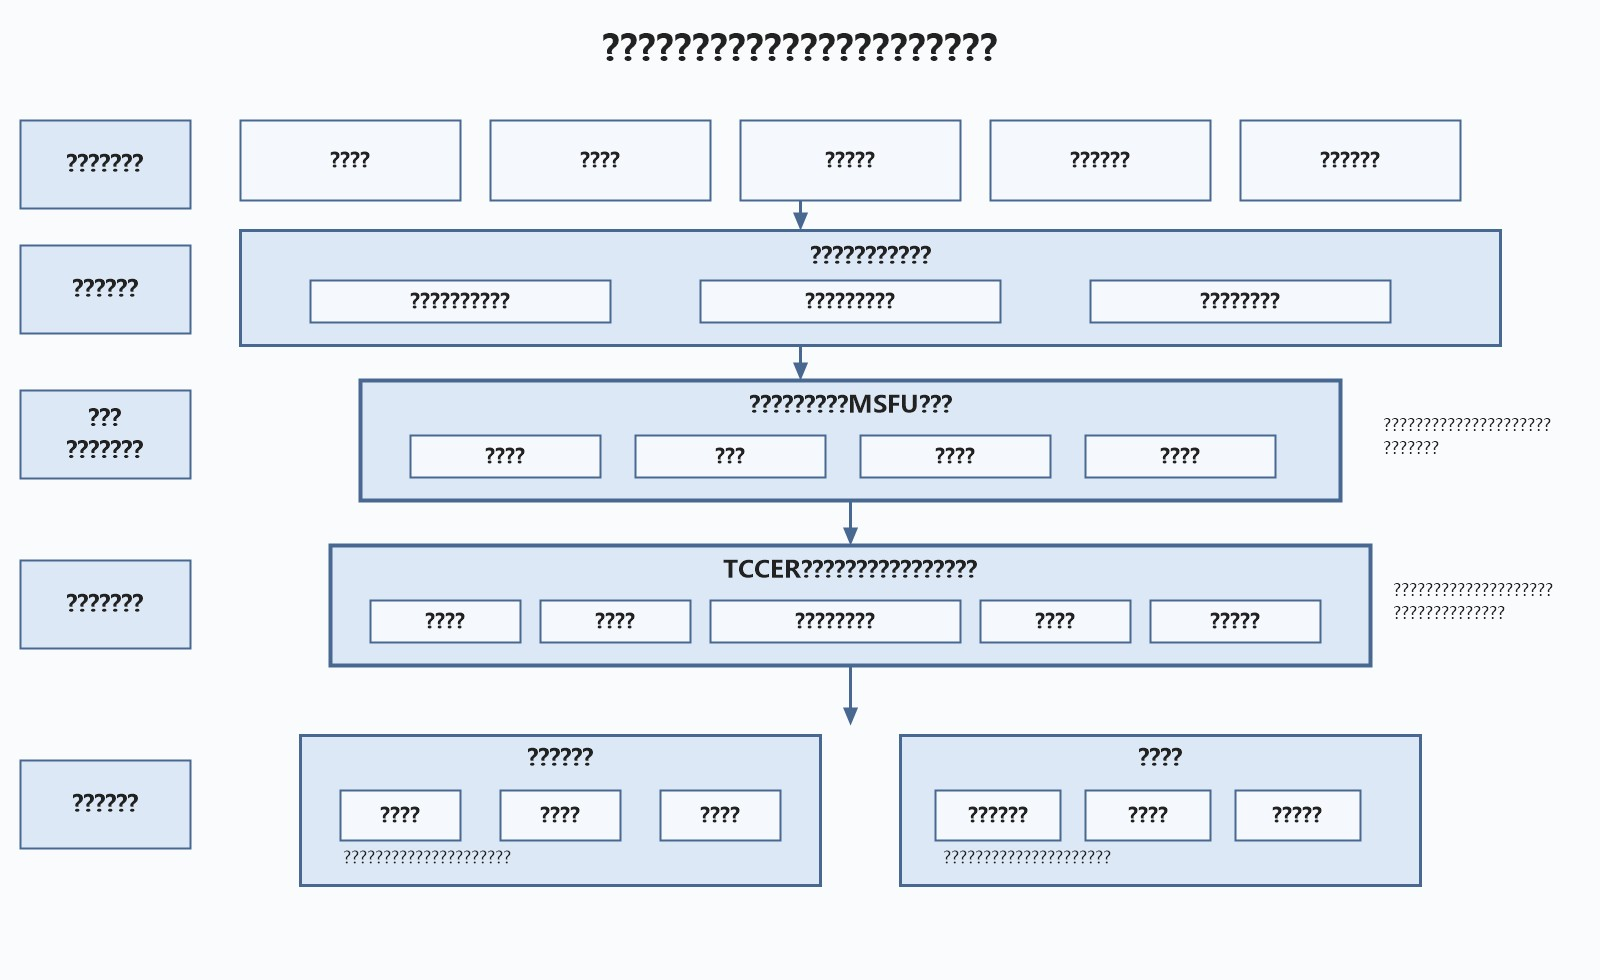
\includegraphics[width=0.95\textwidth]{figures/gemini3.1.jpg}
    \caption{闈㈠悜纰崇撼绫崇闃靛垪鐮旂┒鐨勭煡璇嗗缓妯′笌妫€绱㈠寮烘鏋秨
    \label{fig:3_1}
\end{figure}

\section{闈㈠悜纰崇撼绫崇闃靛垪鐮旂┒鐨勭煡璇嗗崟鍏冨缓妯℃柟娉晑
\ensection{Knowledge Unit Modeling Method for Carbon Nanotube Array Research}

涓烘敮鎾戝悗缁叧绯荤害鏉熸绱€佽瘉鎹仛鍚堜笌鐭ヨ瘑杈呭姪鍒嗘瀽浠诲姟锛岄渶瑕佸皢鏉ユ簮鍒嗘暎銆佸舰寮忓紓鏋勪笖璇箟绮掑害涓嶄竴鑷寸殑鍘熷鐭ヨ瘑杞寲涓虹粺涓€銆佸彲鍏宠仈銆佸彲妫€绱㈢殑缁撴瀯鍖栬〃绀恒€傞拡瀵圭⒊绾崇背绠￠樀鍒楃爺绌朵腑瀛︽湳鏂囩尞銆佸疄楠岃褰曘€佸伐鑹哄弬鏁拌〃銆佺粨鏋勫寲鏁版嵁搴撳強鍥惧儚琛ㄥ緛缁撴灉骞跺瓨鐨勭壒鐐癸紝鏈枃鍥寸粫澶氭簮鐭ヨ瘑瑙勮寖鍖栥€侀潰鍚戠鐮斾簨瀹炵殑灞傛鍖栧垏鍒嗐€佹渶灏忚涔変簨瀹炲崟鍏冩瀯寤轰互鍙婃牳蹇冨璞♀€斿叧绯昏鍒欏缓妯″洓涓柟闈㈠紑灞曠煡璇嗚〃绀虹爺绌讹紝褰㈡垚闈㈠悜纰崇撼绫崇闃靛垪鐮旂┒鐨勭煡璇嗗崟鍏冨缓妯℃柟娉曪紝涓哄悗缁叧绯荤害鏉熸绱笌璇佹嵁鍙拷婧垎鏋愭彁渚涚粺涓€鐨勭粨鏋勫寲鍩虹銆?
\subsection{澶氭簮鐭ヨ瘑瑙勮寖鍖栧鐞唥
\ensubsection{Normalized Processing of Multi-source Knowledge}

纰崇撼绫崇闃靛垪鐮旂┒涓殑鍘熷鐭ヨ瘑鏉ユ簮涓昏鍖呮嫭瀛︽湳鏂囩尞銆佸疄楠岃褰曚笌宸ヨ壓鍙傛暟琛ㄣ€佺粨鏋勫寲瀹為獙鏁版嵁搴撲互鍙婂浘鍍忚〃寰佺粨鏋溿€傚湪姝ゅ墠妗嗘灦鎸囧涓嬶紝鐢变簬涓嶅悓鏉ユ簮鏁版嵁鍦ㄦ枃浠舵牸寮忋€佸瓧娈电粍缁囨柟寮忓拰璇箟琛ㄨ揪绮掑害涓婂瓨鍦ㄦ樉钁楀樊寮傦紝鑻ョ洿鎺ヤ綔涓哄悗缁煡璇嗗缓妯＄殑杈撳叆锛屾瀬鏄撳鑷村悓绫讳俊鎭〃绀轰笉涓€鑷淬€佹牱鍝佹爣璇嗘棤娉曞榻愪互鍙婁笂涓嬫枃璇箟缂哄け绛夐棶棰樸€備负姝わ紝鏈枃璁捐浜嗕竴濂楅潰鍚戝婧愬紓鏋勭煡璇嗙殑瑙勮寖鍖栧鐞嗘祦绋嬶紝灏嗕笉鍚屾潵婧愮煡璇嗙粺涓€杞崲涓虹粨鏋勪竴鑷淬€佸瓧娈垫竻鏅扮殑鏍囧噯鍖栦腑闂磋〃绀恒€?
璁惧師濮嬪婧愮煡璇嗛泦鍚堜负锛?\begin{equation}
    D = \{d_k\}_{k=1}^N
\end{equation}
鍏朵腑锛?d_k$ 琛ㄧず绗?$k$ 涓師濮嬬煡璇嗗璞′釜浣撱€傛湰鏂囬€氳繃瑙勮寖鍖栨槧灏勫嚱鏁?$F_{\mathrm{norm}}(\cdot)$ 灏嗗師濮嬬煡璇嗗璞＄粺涓€杞崲涓鸿鑼冨寲鐭ヨ瘑闆嗗悎 $\tilde{D}$锛?\begin{equation}
    \tilde{d}_k = F_{\mathrm{norm}}(d_k)
\end{equation}
鍏朵腑锛?\tilde{d}_k$ 琛ㄧず缁忚繃鏍煎紡涓庡瓧娈靛榻愬悗鐨勮鑼冨寲鐭ヨ瘑瀵硅薄銆?
閽堝涓嶅悓绫诲瀷鐨勬暟鎹簮锛屾湰鏂囬噰鐢ㄥ樊寮傚寲鐨勮鑼冨寲澶勭悊绛栫暐銆傚浜庡鏈枃鐚紝涓昏鎵ц鐗堝紡鍘诲櫔銆佹湳璇綊涓€鍖栥€佹钀界粨鏋勪繚鐣欏拰鍙傝€冧俊鎭娊鍙栵紝浠ユ渶澶х▼搴︿繚鐣欏惈鏈夊伐鑹烘弿杩般€佸疄楠岀幇璞°€佹満鐞嗗垎鏋愬拰鎬ц兘缁撹鐨勬牳蹇冭涔夋钀斤紱瀵逛簬瀹為獙璁板綍涓庡伐鑹哄弬鏁拌〃锛岄噸鐐瑰洿缁曟牱鍝佺紪鍙枫€佹壒娆＄紪鍙峰拰鏍稿績宸ヨ壓鍙傛暟鎵ц璺ㄨ〃鐨勫瓧娈靛榻愪笌鍛藉悕瑙勮寖锛屾秷闄や釜浜鸿褰曚範鎯甫鏉ョ殑鍚屼箟瀛楁骞叉壈锛涘浜庣粨鏋勫寲瀹為獙鏁版嵁搴擄紝纭珛浠ユ牱鍝佺紪鍙蜂负涓婚敭鐨勫叏灞€缁熶竴绱㈠紩锛屼互澧炲己鍚勭嫭绔嬫暟鎹〃涔嬮棿鐨勮法琛ㄥ叧鑱旇兘鍔涳紱瀵逛簬鍥惧儚琛ㄥ緛缁撴灉锛屽垯涓ユ牸灏嗗浘鍍忓舰璨岀壒寰佸垽瀹氭寚鏍囩粺涓€瑙勮寖涓哄彇鍚戝害銆佸钩鍧囨洸鐜囥€佽鐩栧瘑搴︿笌鐩村緞鍒嗗竷鍥涢」鏍稿績鍙傞噺锛屽苟浣垮叾涓庣浉搴旀壒娆＄殑鏍峰搧鍏冩暟鎹繘琛岀粦瀹氥€?
澶氭簮寮傛瀯鐭ヨ瘑瑙勮寖鍖栧鐞嗘祦绋嬪鍥緙\ref{fig:3_2_norm_flow} 鎵€绀恒€傞€氳繃涓婅堪澶勭悊锛屽绔嬪拰纰庣墖鍖栫殑澶氭簮鏈綋琚垚鍔熻浆鍖栦负楂樺害鍐呰仛鐨勬爣鍑嗚〃杈惧舰寮忋€傝繖涓€瑙勮寖鍖栫粨鏋滀笉浠呬负鍚庣画鐨勬枃鏈眰娆″寲鍒囧垎鎻愪緵浜嗘牸寮忓綊涓€鍖栫殑缁熶竴杈撳叆锛屽悓鏃朵篃涓鸿法鏁版嵁婧愮殑鏍峰搧绾у疄浣撳榻愩€佺粏棰楃矑搴﹀叧绯绘娊鍙栵紝浠ュ強鏈€缁堝眬閮ㄥ叧绯诲瓙鍥剧殑鏈夋晥鏋勫缓鎻愪緵浜嗗潥瀹炵殑鏁版嵁鍩虹銆?
\begin{figure}[H]
    \centering
    \includegraphics[width=0.92\textwidth]{figures/gemini3.2.png}
    \caption{澶氭簮寮傛瀯鐭ヨ瘑鐨勮鑼冨寲澶勭悊娴佺▼绀烘剰鍥緘
    \label{fig:3_2_norm_flow}
\end{figure}

\subsection{闈㈠悜绉戠爺浜嬪疄鐨勫眰娆″寲鍒囧垎鏂规硶}
\ensubsection{Hierarchical Segmentation Method Based on Scientific Facts}

鍦ㄥ畬鎴愬婧愮煡璇嗚鑼冨寲澶勭悊鍚庯紝闇€灏嗛暱鏂囨湰杞崲涓洪€傚悎淇℃伅鎶藉彇鐨勫瓙鐗囨銆傚浜庣⒊绾崇背绠￠樀鍒楃爺绌惰鏂欒€岃█锛屽崟涓枃鏈墖娈典腑寰€寰€娣卞害铻嶅悎浜嗗伐鑹烘潯浠躲€佸疄楠岀幇璞″強鍐呭湪鏈虹悊瑙ｉ噴銆備紶缁熺殑鍩轰簬鍥哄畾闀垮害鎴栨粦鍔ㄧ獥鍙ｇ殑鏅€氬垏鍒嗭紙Chunking锛夋瀬鏄撶牬鍧忓眬閮ㄧ鐮斾簨瀹為摼鏉°€備负鏇村ソ鍦版湇鍔′簬绉戠爺浜嬪疄琛ㄨ揪锛屾湰鏂囪璁′簡涓€绉嶉潰鍚戠鐮斾簨瀹炵殑灞傛鍖栧垏鍒嗘柟娉曪紝鍏舵牳蹇冪洰鏍囨槸鏈€澶ч檺搴﹀湴淇濈暀鏂囨湰涓€滄潯浠垛€旂幇璞♀€旇В閲娾€濈殑灞€閮ㄤ簨瀹為摼瀹屾暣鎬с€?
璁捐鑼冨寲鍚庣殑鐭ヨ瘑瀵硅薄 $\tilde{d}_k$ 瀵瑰簲鏂囨湰鍐呭涓?$x_k$锛屾湰鏂囧紩鍏ヨ瀺鍚堢鐮旈€昏緫杈圭晫鐨勫垎娈垫槧灏勫嚱鏁?$F_{\mathrm{seg}}(\cdot)$锛屽皢鍏惰浆鎹负鍊欓€変簨瀹炵墖娈甸泦鍚?$S_k$锛?\begin{equation}
    S_k = F_{\mathrm{seg}}(x_k) = \{ s_{k,j} \}_{j=1}^{M_k}
\end{equation}
鍏朵腑锛?s_{k,j}$ 琛ㄧず浠庣 $k$ 涓煡璇嗗璞′腑鍒囧垎寰楀埌鐨勭 $j$ 涓€欓€変簨瀹炵墖娈碉紝$M_k$ 琛ㄧず璇ュ璞¤鎷嗗垎鍚庣殑鎬荤墖娈垫暟銆?
璇ュ垏鍒嗘柟娉曚弗鏍奸伒寰€滈珮灞傜粨鏋勮竟鐣屼紭鍏堛€佹绾ц涔夎竟鐣岄€掕繘銆佸眬閮ㄤ笂涓嬫枃閲嶅彔淇濈暀鈥濈殑鍘熷垯浣撶郴銆傞鍏堬紝浼樺厛渚濇嵁娈佃惤鎹㈣銆佸皬鑺傛爣棰樸€佸疄楠屾楠ゅ強鍙傛暟鍒楄〃绛夐珮浼樺厛绾х粨鏋勮竟鐣岃繘琛屽垵濮嬪垝鍒嗭紝閬垮厤鏂╂柇鏍稿績璁鸿堪閫昏緫銆傚叾娆★紝褰撳垵姝ュ垝鍒嗙殑鐗囨闀垮害浠嶈秴杩囬璁剧殑澶ц瑷€妯″瀷鏈€浣冲鐞嗛槇鍊兼椂锛屽垯娌跨敤鍙ュ彿銆佸垎鍙峰強骞跺垪鍙傛暟椤硅竟鐣岀瓑娆＄骇璇箟杈圭晫杩涜閫掑綊缁嗗垎锛屼娇鐗囨鍦ㄦ弧瓒抽暱搴︾害鏉熺殑鍚屾椂淇濇寔灞€閮ㄨ涔夎繛缁€с€傛渶鍚庯紝涓哄噺寮辩‖鎬у垏鍒嗗涓婁笅鏂囨寚浠ｅ叧绯荤殑鐮村潖锛屽湪鐩搁偦鐗囨闂村紩鍏ュ眬閮ㄩ噸鍙犵獥鍙ｃ€傝鍗曠墖娈垫渶澶ч暱搴﹂槇鍊间负 $L_{\max}$锛岀浉閭荤墖娈甸噸鍙犲瓧绗﹂暱搴︿负 $r$锛屽垯璋冩暣鍚庣殑鏈€缁堝垏鍒嗙墖娈?$s_{k,j}'$ 婊¤冻濡備笅闄愬埗鍏崇郴锛?\begin{equation}
    L(s_{k,j}) \leq L_{\max}
\end{equation}
\begin{equation}
    s_{k,j}' = s_{k,j} \cup \mathrm{tail}_{r}(s_{k,j-1})
\end{equation}

涓庝紶缁熷浐瀹氶暱搴︾殑鏂囨湰鍧楀垏鍒嗘ā寮忕浉姣旓紝涓婅堪缁忚繃灞傛鍖栬竟鐣岀害鏉熷鐞嗘墍鑾峰彇鐨勮緭鍑猴紝涓嶅啀鏄浉浜掑壊瑁傜殑鏂囨湰鏁ｅ潡锛岃€屾槸楂樺害鍐呰仛閫昏緫绾跨储鐨勮涔夎浇浣撱€傝繖浜涢珮璐ㄩ噺鐨勫€欓€夌墖娈典笉浠呯洿鎺ユ湇鍔′簬涓嬩竴灏忚妭鏈€灏忚涔変簨瀹炲崟鍏冿紙MSFU锛夌殑鏋勫缓锛屽悓鏃朵篃浣滀负鍧氬疄鐨勬枃鏈€欓€夊熀纭€锛屾湁鍔涙敮鎾戜簡鍚庣画澶ц妯″疄浣撳叧绯绘娊鍙栦笌灞€閮ㄥ叧绯诲瓙鍥炬瀯寤哄伐浣溿€?
\subsection{鏈€灏忚涔変簨瀹炲崟鍏冭〃绀簘
\ensubsection{Representation of Minimum Semantic Fact Unit}

鍦ㄨ幏鍙栬暣鍚眬閮ㄩ€昏緫鐨勫眰娆″寲鐗囨鍚庯紝鑻ヨ鏀拺璺ㄧ淮搴︾殑澶嶆潅绉戝闂鎺ㄧ悊锛屽繀椤昏繘涓€姝ユ墦鐮翠紶缁熼潪缁撴瀯鍖栨枃鏈殑琛ㄨ揪灞€闄愩€備紶缁熺殑鏅€氭枃鏈潡閫氬父浠呮敮鎸佸熀浜庤瘝姹囨垨鍚戦噺琛ㄧず鐨勭浉浼煎害妫€绱紝缂轰箯瀵圭煡璇嗗唴閮ㄥ洜鏋滃叧鑱斾笌闄愬畾绾︽潫鐨勬樉寮忔劅鐭ヨ兘鍔涖€備负瀹炵幇绮剧‘鐨勫叧绯绘函婧愪笌閫昏緫鎺ㄦ紨锛屾湰鏂囨彁鍑篭textbf{鏈€灏忚涔変簨瀹炲崟鍏儅锛圡inimum Semantic Fact Unit, MSFU锛夌殑澶勭悊鑼冨紡銆傝繖涓€杩囩▼鏍囧織鐫€鏁版嵁琛ㄧず鐢辨櫘閫氱殑鏂囨湰鐗囨鍚戠粨鏋勫寲銆佸彲妫€绱㈢鐮斾簨瀹炲崟鍏冪殑鍏抽敭鎻愬崌銆?
鍖哄埆浜庡父瑙勭殑鐭ヨ瘑搴撶墖娈靛垏鐗囷紝鏈€灏忚涔変簨瀹炲崟鍏冩樉寮忕紪鐮佷簡鍙戠敓鍏宠仈鐨勫璞°€佸叧绯绘満鍒躲€佽Е鍙戞潯浠跺強鍘熷璇佹嵁銆傛湰鏂囧皢杩欎竴澶嶅悎鍗曞厓鐨勯珮瑙勯€昏緫琛ㄧず璁惧畾涓哄涓嬬粨鏋勶細
\begin{equation}
    u_{k,j} = (x_{k,j}, \, m_{k,j}, \, r_{k,j}, \, e_{k,j})
\end{equation}
鍦ㄨ妗嗘灦琛ㄧず浣撶郴涓細$x_{k,j}$ 涓鸿鐭ヨ瘑鐨勫師鐢熸枃鏈墖娈佃〃绀猴紱$m_{k,j}$ 鎻愪緵浜嗗寘鍚潵婧愩€佷富棰樼被鍒拰浠诲姟瀵煎悜灞炴€х殑鍏冩暟鎹泦鍚堬紱鍏舵牳蹇冪殑鍔ㄥ姏涓灑涓哄叧绯诲寲璇箟妲戒綅闆?$r_{k,j}$锛涙澶栵紝杈呬互鐢ㄤ簬闃叉妯″瀷骞昏骞舵敮鎾戞函婧愭煡璇佺殑璇佹嵁妲藉崟鍏?$e_{k,j}$銆傝琛ㄧず鏋舵瀯鐨勬柟娉曟剰涔夊湪浜庯細褰诲簳鎽掑純浜嗗皢鏂囨湰浠呬綔涓烘墎骞冲瓧绗﹀簭鍒楃殑澶勭悊鏂瑰紡锛岃祴浜堜簡姣忎竴涓墖娈典互鏄庣‘鐨勯鍩熼€昏緫韬唤鍜屽叧绯讳紶閫掕兘鍔涳紝浠庤€屾瀯绛戜簡缁撴瀯鍖栭€昏緫鎺ㄦ紨鐨勫熀鐭炽€?
杩涗竴姝ュ睍寮€鍒嗘瀽鍏舵牳蹇冨叧绯诲寲璇箟妲戒綅 $r_{k,j}$锛屽叾鍐呴儴鎷撴墤缁勬垚鍏蜂綋濡備笅锛?\begin{equation}
    r_{k,j} = (s_{k,j}, \, t_{k,j}, \, c_{k,j}, \, d_{k,j}, \, q_{k,j})
\end{equation}
杩欎竴缁撴瀯璁捐鐨勬牳蹇冩垬鐣ュ湪浜庝笌鍚庣画妫€绱㈠寮虹畻娉曞缓绔嬪師鐢熺殑鍥捐鎸傛帴閫氶亾銆傚叿浣撹€岃█锛氳捣鍙戣绱?$s_{k,j}$ 锛堟簮瀹炰綋锛変笌鍙椾綔鐢ㄦ柟 $t_{k,j}$ 锛堢洰鏍囧疄浣擄級杩炲悓鍏朵氦浜掔被鍒?$c_{k,j}$ 锛堝叧绯荤被鍨嬶級锛屽湪姒傚康灞傞潰涓婂彲鑷劧鏃犵紳鏄犲皠涓哄悗缁璞″叧绯诲浘璋变腑鐨刓textbf{鑺傜偣涓庤繛杈箎锛涗笌姝ゅ悓鏃讹紝鎻忚堪婕斿彉璧板娍鐨?$d_{k,j}$ 锛堜綔鐢ㄦ柟鍚戯級锛屼弗瀵嗗湀瀹氳寰嬬敓鏁堝墠鎻愮殑 $q_{k,j}$ 锛堟潯浠惰寖鍥达級锛屼互鍙婂墠杩拌瘉鎹Ы涓敤浠ラ獙璇佺殑璇佹嵁鐗囨鏂囨湰鍙婄疆淇″害鍥犲瓙锛屽皢鍏卞悓浣滀负鎸傝浇浜庤鍏崇郴鍥捐繛甯︿笂鐨刓textbf{澶氱淮杈瑰睘鎬э紙Edge Attributes锛墋銆傝繖涓€涓ュ瘑鐨勫弬鏁拌浆鍖栫粍鍚堬紝涓嶄粎纭繚浜嗗绔嬬殑浜嬪疄鐗囨鑳藉浠庢牴鏈笂鍚堣婕斿彉涓哄浘瀹炰綋锛屼粠鑰屼篃涓哄悗缁珮鏁堟墽琛屽眬閮ㄥ叧绯诲瓙鍥剧殑鍙楅檺妫€绱㈡満鍒舵彁渚涗簡缁熶竴鏍囧噯鐨勮〃绀哄熀纭€銆?
涓轰簡绯荤粺鎬у湴璇存槑璇ョ粍缁囩殑鍐呴儴鍔熻兘鍙婂崗鍚屾満鍒讹紝琛▇\ref{tab:3_1_unit_schema} 闃愰噴浜嗚鏈€灏忚涔変簨瀹炲崟鍏冪殑鏍稿績鏋勪欢鍙婂叾鍦ㄦ暣浣撳垎鏋愮绾夸腑鎵€鍙戞尌鐨勪綔鐢ㄥ畾浣嶃€傝繖宸蹭笉鍐嶆槸鍗曠函鐨勬暟鎹簱姒傚康璇存槑锛岃€屾槸涓€灞傛敮鎾戠瀛︽帹鐞嗙殑璁ょ煡楠ㄦ灦銆?
\begin{table}[htbp]
    \centering
    \caption{鏈€灏忚涔変簨瀹炲崟鍏冨瓧娈佃璁″強鍏朵綔鐢ㄨ鏄巬
    \label{tab:3_1_unit_schema}
    \renewcommand{\arraystretch}{1.3}
    \setlength{\tabcolsep}{6pt}
    \begin{tabular}{p{2.5cm} p{5.5cm} p{5.0cm}}
        \toprule
        \textbf{瀛楁绫诲埆} & \textbf{瀛楁缁勬垚} & \textbf{涓昏浣滅敤} \\
        \midrule
        鍏冩暟鎹瓧娈?        & 鏂囨。鏍囪瘑锛坉oc\_id锛夈€佹爣棰橈紙title锛夈€佹潵婧愮被鍨嬶紙source\_type锛夈€佷富棰樼被鍒紙theme锛夈€佷换鍔℃爣绛撅紙task\_tag锛夈€佸勾浠斤紙year锛?
        & 鏀寔鏉ユ簮绮剧‘杩囨护涓庣矖绮掑害涓婚浠诲姟瀹氬悜绾︽潫鎺掓煡 \\
        \midrule
        璇箟瀛楁
        & 婧愬疄浣擄紙source\_entity锛夈€佺洰鏍囧疄浣擄紙target\_entity锛夈€佸叧绯荤被鍨嬶紙relation\_type锛夈€佷綔鐢ㄦ柟鍚戯紙effect\_direction锛夈€佹潯浠惰寖鍥达紙condition\_scope锛?
        & 鏍稿績鏀拺瀵硅薄鍏崇郴缁撴瀯绾︽潫妫€绱€佽矾寰勭瓫閫変笌缁撴瀯鍖栧垎鏋?\\
        \midrule
        鎵╁睍璇箟瀛楁
        & 鏈哄埗鏈锛坢echanism\_terms锛夈€佹€ц兘鏈锛坧erformance\_terms锛?
        & 澧炲己鏈虹悊瑙ｉ噴涓庢€ц兘鍒嗘瀽鍦烘櫙涓嬪簳灞傞€昏緫鐨勭郴缁熸劅鐭ヨ兘鍔?\\
        \midrule
        璇佹嵁瀛楁
        & 璇佹嵁鐗囨锛坋vidence\_span锛夈€佸叧閿瘝锛坘eywords锛夈€佺疆淇″害锛坈onfidence锛夈€佹牳蹇冩€ф爣璁帮紙is\_core锛?
        & 鏀拺鏈€缁堢鐮旇鏂殑缁撴灉楠岃瘉銆佹牳蹇冩煡鎹笌璇佹嵁寮哄害闃蹭吉婧簮 \\
        \bottomrule
    \end{tabular}
\end{table}

\subsection{鏍稿績瀵硅薄銆佸叧绯荤被鍨嬩笌绾︽潫瑙勫垯寤烘ā}
\ensubsection{Modeling of Core Objects, Relation Types, and Constraint Rules}

鍦ㄧ‘绔嬫渶灏忚涔変簨瀹炲崟鍏冭〃绀轰綋绯诲悗锛屼负閬垮厤娴烽噺浜嬪疄鍗曞厓鍦ㄦ绱笌鎺ㄧ悊涓嚭鐜版棤搴忚仛鍚堬紝闇€浠庡叏灞€瑙嗚涓哄叾鎻愪緵楂樺眰娆＄殑鐭ヨ瘑缁勭粐妗嗘灦銆傛湰鐮旂┒缁撳悎纰崇撼绫崇闃靛垪鏉愭枡鐢熼暱鐨勪笓涓氱壒鎬э紝褰掔撼鍑哄洓鏂归潰鏍稿績瀵硅薄涓庝簲澶х被鍏崇郴璺緞锛屽苟杈呬互鐩稿簲鐨勭害鏉熸満鍒躲€傝繖涓夎€呯殑缁撳悎锛屽叡鍚屾瀯寤哄嚭浜嗕竴濂梊textbf{闈㈠悜纰崇撼绫崇闃靛垪鐮旂┒鐨勮交閲忕骇棰嗗煙鍏崇郴缁撴瀯}銆?
棣栧厛锛屾湰绔犲皢澶嶆潅搴炲ぇ涓斿舰鎬佸悇寮傜殑寰瀹炰綋鏈哄埗鍙橀噺鏀舵暃涓哄洓绫绘渶涓烘椿璺冪殑鏍稿績瀵硅薄绫荤皣锛堣琛▇\ref{tab:3_2_entities}锛夛細宸ヨ壓瀹炰綋缁熸嫭娓╁害銆佹皵浣撴祦閲忕瓑璋冩帶鐜鐨勫鍦ㄥ共棰勯噺锛涘舰璨屽疄浣撳垯蹇犲疄钀藉畾浜庨樀鍒楃殑绌洪棿鍙鐗瑰緛锛岀粺涓€鍖呮嫭鍙栧悜搴︺€佸钩鍧囨洸鐜囥€佽鐩栧瘑搴﹀拰鐩村緞鍒嗗竷锛涙€ц兘瀹炰綋涓撻棬娑电洊鏉愭枡鍦ㄧ粓绔簲鐢ㄦ墍鍛堢幇鐨勫鍦ㄦ祴瀹氬弽棣堝睍鐜帮紱鏈虹悊瀹炰綋鍒欒礋璐ｆ繁搴﹀嚌缂╅偅浜涜棌浜庤〃璞′箣涓嬪鑷存紨鍖栫殑娣卞眰寰椹卞姩鐜拌薄銆?
\begin{table}[htbp]
    \centering
    \caption{鏍稿績瀵硅薄绫诲埆鍙婄ず渚嬭鏄巬
    \label{tab:3_2_entities}
    \renewcommand{\arraystretch}{1.3}
    \setlength{\tabcolsep}{6pt}
    \begin{tabular}{p{2.5cm} p{5.5cm} p{5.0cm}}
        \toprule
        \textbf{瀵硅薄绫诲埆} & \textbf{鍏稿瀷绀轰緥} & \textbf{璇存槑} \\
        \midrule
        宸ヨ壓瀹炰綋 & 鐢熼暱娓╁害銆侀€€鐏椂闂淬€佸偓鍖栧墏鍘氬害銆佺紦鍐插眰鍘氬害銆佹皵浣撴祦閲忋€佸偓鍖栧墏鐘舵€?& 鎻忚堪瀹為獙杈撳叆鏉′欢涓庡井瑙傚伐鑹哄共棰勫悇椤硅皟鎺у弬鏁?\\
        \midrule
        褰㈣矊瀹炰綋 & 鍙栧悜搴︺€佸钩鍧囨洸鐜囥€佽鐩栧瘑搴︺€佺洿寰勫垎甯?& 涓ユ牸缁熶竴瀹氫箟纰崇撼绫崇闃靛垪绯荤粺鐨勭┖闂寸粨鏋勪笌寰琛ㄧ幇鐗瑰緛 \\
        \midrule
        鎬ц兘瀹炰綋 & 瀵肩數鎬с€佺數闃荤巼銆佹媺浼稿己搴︺€佸脊鎬фā閲?& 鎻忚堪鐢熸垚鏉愭枡鍦ㄦ渶缁堝疄闄呭簲鐢ㄧ鍛堢幇鐨勫畯瑙傛娴嬫暟鎹〃鐜?\\
        \midrule
        鏈虹悊瀹炰綋 & 鍌寲鍓傚け娲汇€佹墿鏁ｅ彈闄愩€佽竟鐣屽眰鏁堝簲銆侀绮掑洟鑱氥€佸ゥ鏂壒鐡﹀皵寰风啛鍖栥€佸簲鍔涜瀵煎集鏇?& 娴撶缉鎻ず瀵艰嚧鍚勮娴嬮噺鍙戠敓婕斿彉鍒嗗寲鐨勬繁灞傛牳蹇冪墿鐞嗕笌鍖栧杩愪綔鏈哄埗 \\
        \bottomrule
    \end{tabular}
\end{table}

涓洪┍鍔ㄩ潤鎬佸垎绫诲璞＄殑鏈夊簭浼犲锛屾湰鏂囪繘涓€姝ユ娊璞″嚭璐€氬洓澶у疄浣撶被鍒殑浜旂被瀹氬悜鍒嗘瀽澶у姩鑴夛紙濡傚浘~\ref{fig:3_3_schema} 鎵€绀猴級銆傜涓€绫讳负\textbf{宸ヨ壓鈥斿舰璨屽叧绯伙紙process-to-morphology锛墋锛屾弿杩板璁炬帶鍒跺弬閲忓悜鏉愭枡鍑犱綍琛ㄧ幇杞寲鐨勭洿鎺ュ叧鑱旓紱绗簩绫讳负\textbf{褰㈣矊鈥旀€ц兘鍏崇郴锛坢orphology-to-performance锛墋锛岃繛鎺ュ井瑙傞樀鍒楀嚑浣曠粨鏋勫埌鏋侀檺搴旂敤瀹炴晥鐨勪紶瀵兼ˉ姊侊紱绗笁绫讳负\textbf{宸ヨ壓鈥旀€ц兘鍏崇郴锛坧rocess-to-performance锛墋锛屽睘浜庣渷鐣ラ儴鍒嗕腑闂寸幆鑺傜殑榛戠洅棰勬祴蹇垽绾匡紱绗洓绫讳负\textbf{宸ヨ壓鈥旀満鐞嗗叧绯伙紙process-to-mechanism锛墋锛岀敤浠ヨ拷鏈函婧愶紝鎺㈢储瀹忚璋冩帶濡備綍婵€娲诲井瑙傛牴鏈墿鐞嗚寰嬶紱绗簲绫讳负\textbf{鏈虹悊鈥斿舰璨屽叧绯伙紙mechanism-to-morphology锛墋锛岄棴鐜彮绀哄唴闅愭満鍒跺浣曞畾鍨嬭浆鍖栦负鏈€缁堝鍦ㄨ惤鏋溿€傝繖浜旂被鍏崇郴骞茬嚎褰诲簳寤撴竻浜嗗鏉傜殑鐮旀帹閫昏緫璺綉銆?
\begin{figure}[H]
    \centering
    \includegraphics[width=0.92\textwidth]{figures/gemini3.3.png}
    \caption{纰崇撼绫崇闃靛垪鐮旂┒涓殑鏍稿績瀵硅薄銆佸叧绯荤被鍨嬩笌绾︽潫瑙勫垯绀烘剰鍥緘
    \label{fig:3_3_schema}
\end{figure}

涓庢鍚屾椂锛屼负浜嗛槻鑼冨璺虫帹婕斾腑鍑虹幇鏃犳晥娉涘寲鐨勬帹鐞嗗穿濉岀幇璞★紝绯荤粺杩涗竴姝ョ‘绔嬩簡鍥涘ぇ绾︽潫瑙勫垯鍫″瀿锛堣琛▇\ref{tab:3_3_relations_rules}锛夈€傚叿浣撳寘鍚細闄愬畾璺宠穬鎺ㄥ蹇呴』瑕佺鍚堢瀛︽棦瀹氱墿鐞嗗叧鑱旂殑\textbf{閾捐矾绾︽潫瑙勫垯}锛涢檺鍒惰兘閲忎紶閫掑崟鍚戞祦鍔ㄤ互闃叉閫嗗悜閿欒鎺ㄦ柇鐨刓textbf{鏂瑰悜绾︽潫瑙勫垯}锛涗弗浠ゆ弧瓒崇壒瀹氭潯浠堕槇鍊硷紙濡傜壒瀹氭俯搴﹀尯娈碉級鎵嶄簣鍒ゆ柇鏀捐鐨刓textbf{鏉′欢绾︽潫瑙勫垯}锛涗互鍙婃湇浠庨《灞備换鍔″鎺ц矾鐢辨寚浠ゅ垎鍙戠殑\textbf{浠诲姟璋冪敤绾︽潫瑙勫垯}銆?
\begin{table}[htbp]
    \centering
    \caption{鍏崇郴绫诲瀷涓庣害鏉熻鍒欒鏄巬
    \label{tab:3_3_relations_rules}
    \renewcommand{\arraystretch}{1.3}
    \setlength{\tabcolsep}{6pt}
    \begin{tabular}{p{3.0cm} p{5.5cm} p{4.5cm}}
        \toprule
        \textbf{绫诲埆} & \textbf{鍚嶇О} & \textbf{鍚箟涓庣害鏉熻鏄巬 \\
        \midrule
        鍏崇郴绫诲瀷 
        & 浜旂被瀵硅薄闂翠富鍏崇郴锛堣鍥緙\ref{fig:3_3_schema}锛?
        & 鎻忚堪宸ヨ壓銆佸舰璨屻€佹€ц兘銆佹満鐞嗛棿鐨勫叏灞€璇箟鍏崇郴涓庡洜鏋滀紶瀵奸摼 \\
        \midrule
        绾︽潫瑙勫垯 
        & 閾捐矾銆佹柟鍚戙€佹潯浠躲€佷换鍔¤皟鐢ㄧ害鏉熻鍒?
        & 闄愬畾鍏崇郴鏈夋晥璺緞涓庝綔鐢ㄦ潯浠堕槇鍊硷紝涓ユ牸鏀寔鍚庣画瀛愬浘鎵╁睍涓庤矾寰勭瓫閫?\\
        \bottomrule
    \end{tabular}
\end{table}

蹇呴』鐫€閲嶅嚫鏄捐繖濂椾綋绯绘鏋剁殑鏂规硶婕旇繘绾ф剰涔夛細瀹冧滑缁濅笉闄愪簬鏈樁娈靛垵鏈熺殑绠€鍗曞睘鎬ф爣娉ㄥ垎绫伙紝鍦ㄥ叾鍚庣殑鐜妭涓紝瀹冧滑灏嗙洿鎺ヤ笅缃矇娣€鎴愪负鏋佸叾鏍稿績娉曞垯渚濇嵁銆傝繖浜涜鍒欐棦鎸囧鐫€娴烽噺鏁版嵁灞曞紑灞€閮ㄥ叧绯诲瓙鍥剧殑鍙楅檺鎵╁睍锛屽張鎷呭綋椹卞姩鍓斾吉瀛樼湡绛涢€夊鏉傛函婧愯矾寰勭殑鍏抽敭鏍囧昂搴曠嚎锛屾渶缁堜负鐢熸垚鍩轰簬纭畾閾捐矾鐨勪簨瀹炶瘉鎹枃鏈彁渚涗簡鏃犲彲鏇挎崲鐨勭粺涓€搴曞眰琛ㄧず鍩虹銆傝嚦姝わ紝鏁翠釜棰嗗煙鍏崇郴缁撴瀯閮ㄧ讲瀹屾瘯锛岀郴缁熷叿澶囦簡鍚戠壒瀹氬叧鑱旈檺鍒剁害鏉熸绱㈣繘琛屾帰寮曠殑瀹屽叏鑳藉姏銆?
\section{闈㈠悜纰崇撼绫崇闃靛垪鐮旂┒鐨勬绱㈠寮烘柟娉晑
\ensection{Retrieval-Augmented Method for Carbon Nanotube Array Research}

鍦ㄥ畬鎴愬婧愮煡璇嗚鑼冨寲銆佹渶灏忚涔変簨瀹炲崟鍏冭〃绀轰互鍙婃牳蹇冨璞°€佸叧绯荤被鍨嬩笌绾︽潫瑙勫垯寤烘ā鍚庯紝鐭ヨ瘑搴撳凡鍏峰闈㈠悜纰崇撼绫崇闃靛垪鐮旂┒鐨勭粨鏋勫寲琛ㄧず鍩虹銆傜劧鑰岋紝浠呮湁鐭ヨ瘑琛ㄧず浠嶄笉瓒充互鐩存帴鏀拺澶嶆潅鐮旂┒闂涓殑绮惧噯鍒嗘瀽銆傚浜庡伐鑹哄垎鏋愩€佸舰璨岃В閲婂拰棰勬祴缁撴灉璇存槑绛変换鍔¤€岃█锛屾绱㈢郴缁熼渶瑕佽繘涓€姝ュ洿缁曞璞″叧绯汇€佹潯浠剁害鏉熷拰璇佹嵁缁勭粐鏂瑰紡寮€灞曠煡璇嗚皟鐢ㄣ€備负姝わ紝鏈枃鍦ㄧ煡璇嗗缓妯″熀纭€涓婃彁鍑洪潰鍚戠⒊绾崇背绠￠樀鍒楃爺绌剁殑妫€绱㈠寮烘柟娉曪紝鍚庣画灏嗕緷娆′粠鐮旂┒浠诲姟涓庢绱㈤渶姹傚垎鏋愩€佹贩鍚堝彫鍥炪€佸眬閮ㄥ叧绯诲瓙鍥炬墿灞曚笌閲嶆帓搴忥紝浠ュ強鍏崇郴閾剧害鏉熺殑璇佹嵁鑱氬悎涓庣敓鎴愬洓涓柟闈㈠睍寮€璁鸿堪銆?
\subsection{鐮旂┒浠诲姟瀹氫箟涓庢绱㈤渶姹傚垎鏋恾
\ensubsection{Research Task Definition and Retrieval Requirement Analysis}

缁撳悎纰崇撼绫崇闃靛垪鐮旂┒涓殑鍏稿瀷鍦烘櫙锛屾湰鏂囧皢妫€绱㈠寮烘墍鏈嶅姟鐨勬牳蹇冧换鍔″綊绾充负浠ヤ笅涓夌被锛?
\begin{enumerate}
    \item \textbf{宸ヨ壓鍒嗘瀽浠诲姟銆倉  
    璇ョ被浠诲姟涓昏鍏虫敞鐗瑰畾宸ヨ壓鍙傛暟鎴栧伐鑹虹粍鍚堝纰崇撼绫崇闃靛垪褰㈣矊鍜屾€ц兘鐨勫奖鍝嶈寰嬶紝渚嬪娓╁害鍙樺寲瀵瑰彇鍚戝害鐨勫奖鍝嶃€佸偓鍖栧墏鍘氬害鍙樺寲瀵圭洿寰勫垎甯冪殑浣滅敤锛屼互鍙婁笉鍚屾皵娴佹瘮鏉′欢涓嬭鐩栧瘑搴︾殑鍙樺寲绛夈€傚浜庢绫讳换鍔★紝妫€绱㈢粨鏋滃簲鑳藉鍑嗙‘鍏宠仈鐩爣宸ヨ壓鍙橀噺涓庡舰璨岀壒寰佹垨鎬ц兘鎸囨爣锛屽苟灏藉彲鑳戒繚鐣欎綔鐢ㄦ柟鍚戙€佹潯浠惰寖鍥村拰璇佹嵁鏉ユ簮绛夊叧閿俊鎭紝浠ユ敮鎸佸弬鏁版瘮杈冦€佽寰嬪綊绾冲拰宸ヨ壓浼樺寲鍒嗘瀽銆?
    \item \textbf{褰㈣矊瑙ｉ噴浠诲姟銆倉  
    璇ョ被浠诲姟涓昏閽堝瀹為獙瑙傛祴鍒扮殑褰㈣矊鐜拌薄锛屽垎鏋愬叾娼滃湪鎴愬洜鍙婄浉鍏虫満鐞嗭紝渚嬪瑕嗙洊瀵嗗害涓嬮檷鍙兘瀵瑰簲鐨勬満鐞嗗彉鍖栥€佸钩鍧囨洸鐜囧澶ф槸鍚︿笌纰充緵缁欎笉鍧囨湁鍏筹紝浠ュ強鍙栧悜搴﹂檷浣庢槸鍚︿笌鍌寲鍓傚け娲绘垨鎵╂暎鍙楅檺鐩稿叧绛夈€備笌宸ヨ壓鍒嗘瀽浠诲姟鐩告瘮锛屽舰璨岃В閲婁换鍔℃洿寮鸿皟宸ヨ壓鍙傛暟銆佺敓闀挎満鐞嗗拰褰㈣矊鐗瑰緛涔嬮棿鐨勯摼寮忔敮鎾戯紝鍥犳妫€绱㈢粨鏋滀笉浠呭簲鍏锋湁璇箟鐩稿叧鎬э紝杩樺簲鍏锋湁杈冨ソ鐨勯摼璺畬鏁存€у拰缁撴瀯涓€鑷存€с€?
    \item \textbf{棰勬祴瑙ｉ噴浠诲姟銆倉  
    璇ョ被浠诲姟闈㈠悜绗洓绔犱腑鐨勫舰璨岄娴嬬粨鏋滐紝鍏虫敞濡備綍鍒╃敤棰嗗煙鐭ヨ瘑瀵规ā鍨嬭緭鍑鸿繘琛岃緟鍔╄鏄庝笌鍚堢悊鎬у垎鏋愩€備緥濡傦紝褰撴ā鍨嬮娴嬫煇缁勫伐鑹哄弬鏁颁笅鍙栧悜搴︿笅闄嶃€佸钩鍧囨洸鐜囧澶ф垨鐩村緞鍒嗗竷澧炲鏃讹紝闇€瑕佽繘涓€姝ヨ鏄庤棰勬祴瓒嬪娍鏄惁鑳藉浠庡凡鏈夊疄楠岃寰嬨€佺敓闀挎満鐞嗘垨鏂囩尞璇佹嵁涓幏寰楁敮鎸併€傛绫讳换鍔′笉浠呰姹傛绱㈢粨鏋滀笌鐩爣宸ヨ壓鍙傛暟鍜岀洰鏍囧舰璨岀壒寰佷繚鎸佷竴鑷达紝杩樿兘澶熸寜鐓р€滃伐鑹哄弬鏁扳€旂敓闀挎満鐞嗏€斿舰璨岀壒寰佲€濇垨鈥滃伐鑹哄弬鏁扳€斿舰璨岀壒寰佲€旀潗鏂欐€ц兘鈥濈瓑涓婚摼杩涜缁勭粐锛屼粠鑰屽舰鎴愬彲楠岃瘉鐨勫叧绯婚摼寮忚瘉鎹€?\end{enumerate}

鍩轰簬涓婅堪浠诲姟鍒掑垎锛屾湰鏂囪涓洪潰鍚戠⒊绾崇背绠￠樀鍒楃爺绌剁殑妫€绱㈠寮烘柟娉曞簲婊¤冻浠ヤ笅涓夋柟闈㈤渶姹傘€傚叾涓€锛屽湪妫€绱㈠璞″眰闈紝搴斾互鏈€灏忚涔変簨瀹炲崟鍏冭€岄潪鏅€氭枃鏈墖娈典綔涓哄熀鏈彫鍥炲璞★紝浠ヤ繚璇佸€欓€夌粨鏋滃叿澶囨槑纭殑瀵硅薄鍏崇郴銆佹潯浠惰寖鍥村拰璇佹嵁淇℃伅銆傚叾浜岋紝鍦ㄦ绱㈣繃绋嬪眰闈紝涓嶅簲浠呬緷璧栨枃鏈浉浼煎害杩涜鍊欓€夋帓搴忥紝杩樺簲杩涗竴姝ョ粨鍚堝璞″叧绯汇€佹潯浠剁害鏉熷拰浠诲姟绫诲瀷杩涜鍙楅檺鎵╁睍涓庤矾寰勭瓫閫夛紝浠ュ寮洪摼璺畬鏁存€у拰浠诲姟鍖归厤鎬с€傚叾涓夛紝鍦ㄦ绱㈣緭鍑哄眰闈紝缁撴灉涓嶅簲鍙槸鑻ュ共绂绘暎鍊欓€夌墖娈电殑闆嗗悎锛岃€屽簲鑳藉杩涗竴姝ョ粍缁囦负灞€閮ㄨ瘉鎹瓙鍥炬垨鍏崇郴閾惧紡璇佹嵁闆嗗悎锛屼互鏀寔澶嶆潅绉戠爺闂涓殑瑙勫緥褰掔撼銆佹満鐞嗚В閲婂拰棰勬祴缁撴灉璇存槑銆?
鍥犳锛屾湰鏂囧悗缁皢棣栧厛鍦ㄦ渶灏忚涔変簨瀹炲崟鍏冨熀纭€涓婃瀯寤烘贩鍚堝彫鍥炴柟娉曪紝浠ヨ幏寰椾笌鏌ヨ鐩稿叧鐨勫€欓€変簨瀹炲崟鍏冿紱闅忓悗锛屽紩鍏ュ眬閮ㄥ叧绯诲瓙鍥炬墿灞曚笌閲嶆帓搴忔満鍒讹紝浠ュ寮哄鏉傜鐮旈棶棰樹腑鐨勯摼璺畬鏁存€т笌瑙ｉ噴涓€鑷存€э紱鏈€鍚庯紝鍥寸粫棰勬祴瑙ｉ噴鍦烘櫙鏋勫缓鍏崇郴閾剧害鏉熺殑璇佹嵁鑱氬悎涓庣敓鎴愭柟娉曪紝涓烘ā鍨嬭緭鍑烘彁渚涘彲杩芥函銆佸彲楠岃瘉鐨勭煡璇嗘敮鎾戙€?
\subsection{鍩轰簬鏈€灏忚涔変簨瀹炲崟鍏冪殑娣峰悎鍙洖鏂规硶}
\ensubsection{Hybrid Retrieval Method Based on Minimum Semantic Fact Units}

鍦ㄥ畬鎴愮爺绌朵换鍔″垝鍒嗕笌妫€绱㈤渶姹傚垎鏋愬悗锛岄鍏堥渶瑕佽В鍐崇殑闂鏄浣曚粠鐭ヨ瘑搴撲腑楂樻晥鍙洖涓庢煡璇㈢浉鍏崇殑鍊欓€変簨瀹炲崟鍏冦€傚浜庣⒊绾崇背绠￠樀鍒楃爺绌朵腑鐨勫伐鑹哄垎鏋愩€佸舰璨岃В閲婂拰棰勬祴瑙ｉ噴浠诲姟鑰岃█锛岃嫢浠呴噰鐢ㄥ崟涓€妫€绱㈡柟寮忥紝寰€寰€闅句互鍏奸【鍙洖瑕嗙洊鐜囦笌缁撴灉绮剧‘鎬с€備竴鏂归潰锛屽熀浜庡叧閿瘝鍖归厤鐨勭█鐤忔绱㈣兘澶熻緝濂戒繚鐣欓鍩熸湳璇€佸伐鑹哄弬鏁扮鍙峰強瀹炰綋鍚嶇О鐨勭簿纭尮閰嶈兘鍔涳紝浣嗗璇箟杩戜技琛ㄨ揪鍜岄殣寮忓叧绯荤殑璇嗗埆鑳藉姏鏈夐檺锛涘彟涓€鏂归潰锛屽熀浜庡悜閲忕浉浼煎害鐨勭瀵嗘绱㈣兘澶熷湪涓€瀹氱▼搴︿笂鎹曟崏璇箟鐩稿叧鎬э紝浣嗗浜庝笓涓氭湳璇€佹暟鍊兼潯浠跺拰棰嗗煙缂╁啓鐨勫尯鍒嗚兘鍔涚浉瀵逛笉瓒筹紝瀹规槗寮曞叆璇箟鐩歌繎浣嗕换鍔′笉鍖归厤鐨勫啑浣欑粨鏋溿€傚洜姝わ紝鏈枃鍦ㄦ渶灏忚涔変簨瀹炲崟鍏冭〃绀哄熀纭€涓婏紝鏋勫缓闈㈠悜纰崇撼绫崇闃靛垪鐮旂┒鐨勬贩鍚堝彫鍥炴柟娉曪紝浠ユ彁鍗囧€欓€変簨瀹炲崟鍏冪殑瑕嗙洊鑳藉姏涓庣浉鍏虫€ц川閲忋€?
璁剧敤鎴锋煡璇㈣涓?$q$锛岀煡璇嗗簱涓殑鏈€灏忚涔変簨瀹炲崟鍏冮泦鍚堣涓?\begin{equation}
U=\{u_i\}_{i=1}^{N}
\end{equation}
鍏朵腑锛?u_i$ 琛ㄧず绗?$i$ 涓渶灏忚涔変簨瀹炲崟鍏冦€傛湰鏂囧垎鍒瀯寤哄熀浜庣█鐤忚〃绀虹殑鍙洖鍑芥暟 $R_{\mathrm{sparse}}(\cdot)$ 鍜屽熀浜庣瀵嗚〃绀虹殑鍙洖鍑芥暟 $R_{\mathrm{dense}}(\cdot)$锛屽苟灏嗕袱鑰呯粨鏋滆繘琛岃瀺鍚堬紝寰楀埌鍊欓€夐泦鍚?$C(q)$锛?\begin{equation}
C(q)=R_{\mathrm{sparse}}(q,U)\cup R_{\mathrm{dense}}(q,U)
\end{equation}

鍏朵腑锛岀█鐤忔绱富瑕侀潰鍚戝叧閿瘝銆佹湳璇拰瀹炰綋绾у尮閰嶏紝绋犲瘑妫€绱富瑕侀潰鍚戣涔夌骇鐩稿叧鎬у彫鍥炪€傞€氳繃浜岃€呯粨鍚堬紝鍙湪淇濊瘉绮剧‘鍖归厤鑳藉姏鐨勫悓鏃跺寮哄璇箟鐩稿叧鐭ヨ瘑鍗曞厓鐨勮鐩栬兘鍔涖€?
瀵逛簬绋€鐤忓彫鍥為儴鍒嗭紝鏈枃浠ユ渶灏忚涔変簨瀹炲崟鍏冧腑鐨勬枃鏈唴瀹广€佸疄浣撳悕绉般€佸叧绯荤被鍨嬪強鍏抽敭璇嶅瓧娈典负涓昏绱㈠紩瀵硅薄锛屾瀯寤哄熀浜庤瘝椤瑰尮閰嶇殑妫€绱㈣〃绀恒€傜敱浜庣⒊绾崇背绠￠樀鍒楃爺绌朵腑瀛樺湪澶ч噺宸ヨ壓鍙傛暟鍚嶇О銆佹満鐞嗘湳璇€佸舰璨屾寚鏍囧拰鎬ц兘鏈锛岀█鐤忔绱㈣兘澶熻緝濂藉湴淇濈暀杩欎簺鏄惧紡绗﹀彿淇℃伅銆備緥濡傦紝褰撴煡璇㈡秹鍙娾€滄俯搴︹€濃€滃彇鍚戝害鈥濃€滃偓鍖栧墏澶辨椿鈥濈瓑鏄庣‘鏈鏃讹紝绋€鐤忔绱㈣兘澶熶紭鍏堝彫鍥炲寘鍚浉鍚屾垨楂樺害涓€鑷存湳璇殑鐭ヨ瘑鍗曞厓锛屼粠鑰屼繚璇佸疄浣撲笌姒傚康灞傞潰鐨勫尮閰嶇簿搴︺€?
瀵逛簬绋犲瘑鍙洖閮ㄥ垎锛屾湰鏂囧皢鏌ヨ $q$ 鍜屾渶灏忚涔変簨瀹炲崟鍏?$u_i$ 鏄犲皠鍒扮粺涓€鐨勫悜閲忕┖闂翠腑銆傝鏌ヨ鍚戦噺琛ㄧず涓?$\mathbf{h}_q$锛岀煡璇嗗崟鍏冨悜閲忚〃绀轰负 $\mathbf{h}_i$锛屽垯浜岃€呯殑璇箟鐩镐技搴﹀彲琛ㄧず涓?\begin{equation}
S_{\mathrm{dense}}(q,u_i)=\cos(\mathbf{h}_q,\mathbf{h}_i)
\end{equation}
鍏朵腑锛?\cos(\cdot,\cdot)$ 琛ㄧず浣欏鸡鐩镐技搴︺€傜瀵嗗彫鍥炶兘澶熸洿濂藉湴鎹曟崏涓嶅悓琛ㄨ堪鏂瑰紡涓嬬殑娼滃湪璇箟涓€鑷存€с€備緥濡傦紝褰撴煡璇娇鐢ㄢ€滅敓闀挎潯浠跺彉鍖栧紩璧烽樀鍒楀集鏇插寮衡€濊€岀煡璇嗗崟鍏冧腑瀵瑰簲鎻忚堪涓衡€滃钩鍧囨洸鐜囧澶т笌宸ヨ壓鎵板姩鐩稿叧鈥濇椂锛岀瀵嗚〃绀鸿兘澶熷湪涓€瀹氱▼搴︿笂寤虹珛涓よ€呬箣闂寸殑璇箟鑱旂郴锛屼粠鑰屽讥琛ョ函鍏抽敭璇嶆绱㈠湪琛ㄨ揪澶氭牱鎬т笂鐨勪笉瓒炽€?
鍦ㄨ幏寰楃█鐤忓彫鍥炵粨鏋滀笌绋犲瘑鍙洖缁撴灉鍚庯紝鏈枃杩涗竴姝ラ噰鐢ㄥ姞鏉冭瀺鍚堢瓥鐣ヨ绠楃煡璇嗗崟鍏冪殑鍒濆鍙洖寰楀垎銆傝 $S_{\mathrm{sparse}}(q,u_i)$ 琛ㄧず鏌ヨ涓庣煡璇嗗崟鍏冧箣闂寸殑绋€鐤忓尮閰嶅緱鍒嗭紝$S_{\mathrm{dense}}(q,u_i)$ 琛ㄧず瀵瑰簲鐨勭瀵嗙浉浼煎害寰楀垎锛屽垯铻嶅悎寰楀垎瀹氫箟涓?\begin{equation}
S_{\mathrm{hybrid}}(q,u_i)=\alpha S_{\mathrm{sparse}}(q,u_i)+(1-\alpha)S_{\mathrm{dense}}(q,u_i)
\end{equation}
鍏朵腑锛?\alpha \in [0,1]$ 琛ㄧず铻嶅悎鏉冮噸锛岀敤浜庡钩琛＄█鐤忓尮閰嶄笌璇箟鐩镐技鎬х殑褰卞搷銆傛渶缁堬紝鎸夌収 $S_{\mathrm{hybrid}}(q,u_i)$ 瀵瑰€欓€夌煡璇嗗崟鍏冭繘琛屾帓搴忥紝骞堕€夊彇鍓?$K$ 涓粨鏋滀綔涓烘贩鍚堝彫鍥炶緭鍑猴細
\begin{equation}
C_K(q)=\operatorname{TopK}\left(S_{\mathrm{hybrid}}(q,u_i)\right)
\end{equation}

涓庝紶缁熼潰鍚戞枃鏈潡鐨勬贩鍚堟绱笉鍚岋紝鏈枃鐨勬贩鍚堝彫鍥炲璞″苟闈炴櫘閫氭枃鏈墖娈碉紝鑰屾槸鏈€灏忚涔変簨瀹炲崟鍏冦€傜敱浜庝簨瀹炲崟鍏冧腑宸叉樉寮忓寘鍚簮瀹炰綋銆佺洰鏍囧疄浣撱€佸叧绯荤被鍨嬨€佹潯浠惰寖鍥村拰璇佹嵁鐗囨绛夊瓧娈典俊鎭紝鍥犳鍙洖缁撴灉涓嶄粎鍏锋湁鏂囨湰鐩稿叧鎬э紝杩樺叿澶囦竴瀹氱殑缁撴瀯鍖栬涔夊熀纭€銆傝繖绉嶈璁′娇寰楀悗缁绱㈣繃绋嬭兘澶熻繘涓€姝ュ洿缁曞璞″叧绯诲拰鏉′欢绾︽潫寮€灞曡矾寰勬墿灞曪紝鑰屼笉蹇呴噸鏂颁粠鍘熷鏂囨湰涓娊鍙栧叧绯讳俊鎭€傛崲瑷€涔嬶紝娣峰悎鍙洖闃舵鐨勭洰鏍囦笉鏄竴娆℃€х粰鍑烘渶缁堢瓟妗堬紝鑰屾槸鍦ㄤ繚璇佽鐩栫巼鐨勫墠鎻愪笅锛屼负鍚庣画灞€閮ㄥ叧绯诲瓙鍥炬墿灞曚笌璇佹嵁閲嶇粍鎻愪緵楂樿川閲忓€欓€変簨瀹炲崟鍏冮泦鍚堛€?
姝ゅ锛岄拡瀵逛笉鍚岀被鍨嬬殑鐮旂┒浠诲姟锛屾湰鏂囧湪鍙洖闃舵杩樺紩鍏ヤ换鍔℃劅鐭ョ殑瀛楁渚ч噸绛栫暐銆傚浜庡伐鑹哄垎鏋愪换鍔★紝浼樺厛寮哄寲宸ヨ壓鍙傛暟瀹炰綋銆佸舰璨屾寚鏍囧拰鎬ц兘鏈鐨勫尮閰嶏紱瀵逛簬褰㈣矊瑙ｉ噴浠诲姟锛屼紭鍏堝己鍖栧舰璨屽疄浣撲笌鏈虹悊鏈涔嬮棿鐨勭浉鍏虫€э紱瀵逛簬棰勬祴瑙ｉ噴浠诲姟锛屽垯鍚屾椂鑰冭檻鐩爣宸ヨ壓鍙傛暟銆佺洰鏍囧舰璨岀壒寰佸強鍏跺彉鍖栨柟鍚戯紝浠ユ彁楂樺€欓€夌粨鏋滀笌寰呰В閲婇棶棰樹箣闂寸殑涓€鑷存€с€傞€氳繃杩欑浠诲姟鎰熺煡鐨勫彫鍥炵瓥鐣ワ紝娣峰悎鍙洖缁撴灉鑳藉鏇村ソ鍦版湇鍔′簬鍚庣画灞€閮ㄥ叧绯诲瓙鍥炬瀯寤哄拰鍏崇郴閾剧害鏉熻瘉鎹敓鎴愩€?
缁间笂锛屾湰鏂囨瀯寤虹殑鍩轰簬鏈€灏忚涔変簨瀹炲崟鍏冪殑娣峰悎鍙洖鏂规硶锛岀患鍚堝埄鐢ㄤ簡绋€鐤忔绱㈢殑绮剧‘鍖归厤鑳藉姏涓庣瀵嗘绱㈢殑璇箟娉涘寲鑳藉姏锛屽湪鎻愬崌鍊欓€変簨瀹炲崟鍏冨彫鍥炶川閲忕殑鍚屾椂锛屼负鍚庣画灞€閮ㄥ叧绯诲瓙鍥炬墿灞曘€佽矾寰勭害鏉熼噸鎺掑簭浠ュ強鍏崇郴閾捐瘉鎹敓鎴愬瀹氫簡鍩虹銆?
\subsection{灞€閮ㄥ叧绯诲瓙鍥炬墿灞曚笌閲嶆帓搴忔柟娉晑
\ensubsection{Local Relationship Subgraph Expansion and Re-ranking Method}

鍦ㄥ熀浜庢渶灏忚涔変簨瀹炲崟鍏冪殑娣峰悎鍙洖闃舵锛屾绱㈢郴缁熷凡缁忚兘澶熻幏寰椾笌鏌ヨ鐩稿叧鐨勫€欓€変簨瀹炲崟鍏冮泦鍚堛€傜劧鑰岋紝瀵逛簬褰㈣矊瑙ｉ噴鍜岄娴嬭В閲婄瓑澶嶆潅鐮旂┒闂鑰岃█锛屼粎渚濊禆鍊欓€変簨瀹炲崟鍏冪殑鍒濆鐩稿叧鎬ф帓搴忎粛瀛樺湪鏄庢樉涓嶈冻銆備竴鏂归潰锛屾贩鍚堝彫鍥炵粨鏋滆櫧鐒惰兘澶熻鐩栦笌鏌ヨ璇箟鐩稿叧鐨勭煡璇嗗崟鍏冿紝浣嗚繖浜涘崟鍏冨線寰€浠嶇劧鏄鏁ｇ殑锛岀己涔忔樉寮忛摼璺粍缁囷紱鍙︿竴鏂归潰锛屽浜庨渶瑕佹満鐞嗚В閲婃垨璇佹嵁鏀拺鐨勯棶棰橈紝鐮旂┒鑰呭叧娉ㄧ殑閫氬父涓嶆槸鍗曟潯浜嬪疄锛岃€屾槸鐢卞伐鑹哄弬鏁般€佹満鐞嗗疄浣撱€佸舰璨岀壒寰佸拰鏉愭枡鎬ц兘绛夊璞℃墍鏋勬垚鐨勫眬閮ㄥ叧绯婚摼銆傝嫢鍊欓€夌粨鏋滀箣闂存棤娉曢€氳繃瀵硅薄鍏崇郴鏈夋晥杩炴帴锛屽垯鍗充娇鍗曟潯浜嬪疄鍏锋湁杈冮珮鐩稿叧鎬э紝涔熼毦浠ョ洿鎺ユ敮鎾戝悗缁В閲婂垎鏋愩€備负姝わ紝鏈枃鍦ㄦ贩鍚堝彫鍥炵粨鏋滃熀纭€涓婏紝杩涗竴姝ユ彁鍑哄眬閮ㄥ叧绯诲瓙鍥炬墿灞曚笌閲嶆帓搴忔柟娉曪紝閫氳繃娌垮璞″叧绯昏繘琛屽彈闄愭墿灞曪紝鏋勫缓涓庢煡璇㈢浉鍏崇殑灞€閮ㄨ瘉鎹瓙鍥撅紝骞剁粨鍚堜换鍔￠渶姹傚鍊欓€夊瓙鍥捐繘琛岄噸鎺掑簭銆?
璁剧敱鐭ヨ瘑鍗曞厓鏄犲皠褰㈡垚鐨勮交閲忕骇棰嗗煙鍏崇郴缁撴瀯琛ㄧず涓?\begin{equation}
G=(V,E)
\end{equation}
鍏朵腑锛?V$ 琛ㄧず瀵硅薄鑺傜偣闆嗗悎锛屽寘鍚伐鑹哄疄浣撱€佸舰璨屽疄浣撱€佹満鐞嗗疄浣撳拰鎬ц兘瀹炰綋锛?E$ 琛ㄧず鍏崇郴杈归泦鍚堬紝姣忔潯杈瑰搴斾竴涓垨澶氫釜鏈€灏忚涔変簨瀹炲崟鍏冿紝骞堕檮甯﹀叧绯荤被鍨嬨€佷綔鐢ㄦ柟鍚戙€佹潯浠惰寖鍥淬€佽瘉鎹墖娈靛拰缃俊搴︾瓑灞炴€с€?
鍦ㄧ粰瀹氭煡璇?$q$ 鐨勬潯浠朵笅锛岃鐢辨贩鍚堝彫鍥為樁娈佃幏寰楃殑鍊欓€変簨瀹炲崟鍏冮泦鍚堜负
\begin{equation}
C_K(q)=\{u_i\}_{i=1}^{K}
\end{equation}
鏈枃棣栧厛灏嗗€欓€変簨瀹炲崟鍏冩槧灏勪负鍏崇郴鍥句腑鐨勭瀛愯竟闆嗗悎锛屽苟浠ヤ笌杩欎簺杈瑰叧鑱旂殑瀹炰綋鑺傜偣浣滀负灞€閮ㄦ墿灞曡捣鐐广€傞殢鍚庯紝鏍规嵁鏍稿績瀵硅薄涔嬮棿鐨勫叧绯荤被鍨嬩笌绾︽潫瑙勫垯锛屽湪鍥剧粨鏋勪腑鎵ц鍙楅檺鎵╁睍锛屾瀯寤轰笌鏌ヨ鐩稿叧鐨勫眬閮ㄥ叧绯诲瓙鍥俱€傝鐢辨煇涓€绉嶅瓙杈?$e_i$ 鎵╁睍寰楀埌鐨勫眬閮ㄥ瓙鍥句负 $G_i^{\mathrm{local}}$锛屽垯鍙涓?\begin{equation}
G_i^{\mathrm{local}}=(V_i^{\mathrm{local}},E_i^{\mathrm{local}})
\end{equation}
鍏朵腑锛?V_i^{\mathrm{local}} \subseteq V$锛?E_i^{\mathrm{local}} \subseteq E$銆?
涓洪伩鍏嶅浘鎵╁睍杩囩▼涓紩鍏ユ棤鍏宠妭鐐瑰拰鍐椾綑閾捐矾锛屾湰鏂囧湪灞€閮ㄥ瓙鍥炬瀯寤鸿繃绋嬩腑寮曞叆浠ヤ笅涓夌被绾︽潫銆傞鍏堟槸\textbf{鍏崇郴绫诲瀷绾︽潫}锛屽嵆浠呭厑璁告部宸ヨ壓鈥斿舰璨屽叧绯汇€佸伐鑹衡€旀満鐞嗗叧绯汇€佹満鐞嗏€斿舰璨屽叧绯汇€佸舰璨屸€旀€ц兘鍏崇郴鍜屽伐鑹衡€旀€ц兘鍏崇郴绛夐瀹氫箟涓诲叧绯昏繘琛屾墿灞曪紝鎺掗櫎涓庣爺绌朵换鍔℃棤鐩存帴鍏宠仈鐨勮竟銆傚叾娆℃槸\textbf{璺緞闀垮害绾︽潫}锛屽嵆闄愬畾灞€閮ㄦ墿灞曠殑鏈€澶ц烦鏁颁负 $H$锛屼互鎺у埗瀛愬浘瑙勬ā骞朵紭鍏堜繚鐣欏眬閮ㄨ瘉鎹摼銆傝浠庣瀛愯竟鍑哄彂鐨勬墿灞曡矾寰勪负 $p$锛屽叾闀垮害璁颁负 $|p|$锛屽垯闇€婊¤冻
\begin{equation}
|p| \leq H
\end{equation}
鍦ㄦ湰鏂囩殑鐮旂┒鍦烘櫙涓紝$H$ 涓€鑸彇 $2$ 鎴?$3$锛屼互淇濊瘉灞€閮ㄥ瓙鍥捐兘澶熻鐩栤€滃伐鑹哄弬鏁扳€旂敓闀挎満鐞嗏€斿舰璨岀壒寰佲€濇垨鈥滃伐鑹哄弬鏁扳€斿舰璨岀壒寰佲€旀潗鏂欐€ц兘鈥濈瓑鏍稿績閾捐矾銆傛渶鍚庢槸\textbf{鏉′欢涓€鑷存€х害鏉焳锛屽嵆鍦ㄦ墿灞曡繃绋嬩腑浼樺厛淇濈暀涓庢煡璇腑宸ヨ壓鏉′欢銆佺洰鏍囧舰璨屾寚鏍囧拰鍙樺寲鏂瑰悜鐩镐竴鑷寸殑鍏崇郴杈癸紝鍑忓皯鏉′欢鍐茬獊甯︽潵鐨勫啑浣欐墿灞曘€?
鍦ㄧ害鏉熸墿灞曞熀纭€涓婏紝鏈枃杩涗竴姝ラ拡瀵逛笉鍚屼换鍔℃瀯寤哄眬閮ㄥ叧绯诲瓙鍥俱€傚浜庡伐鑹哄垎鏋愪换鍔★紝浼樺厛淇濈暀鐢卞伐鑹哄疄浣撳嚭鍙戝苟鎸囧悜褰㈣矊瀹炰綋鎴栨€ц兘瀹炰綋鐨勫眬閮ㄥ瓙鍥撅紝浠ョ獊鍑哄伐鑹哄弬鏁扮殑浣滅敤瑙勫緥锛涘浜庡舰璨岃В閲婁换鍔★紝浼樺厛淇濈暀鍖呭惈宸ヨ壓瀹炰綋銆佹満鐞嗗疄浣撳拰褰㈣矊瀹炰綋鐨勯摼寮忓瓙鍥撅紝浠ュ寮哄瀹為獙鐜拌薄鐨勬満鐞嗘敮鎾戯紱瀵逛簬棰勬祴瑙ｉ噴浠诲姟锛屽垯浼樺厛鏋勫缓鍥寸粫鐩爣宸ヨ壓鍙傛暟鍜岀洰鏍囧舰璨岀壒寰佸睍寮€鐨勪富閾惧瓙鍥撅紝涓哄悗缁叧绯婚摼绾︽潫璇佹嵁鐢熸垚鎻愪緵缁撴瀯鍖栧熀纭€銆?
鍦ㄨ幏寰楀€欓€夊眬閮ㄥ瓙鍥惧悗锛屾湰鏂囪繘涓€姝ヨ璁￠噸鎺掑簭鏈哄埗锛屽鍏惰繘琛屼换鍔℃劅鐭ョ殑缁煎悎璇勫垎銆傝灞€閮ㄥ瓙鍥?$G_i^{\mathrm{local}}$ 鐨勭患鍚堝緱鍒嗕负 $S_{\mathrm{graph}}(q,G_i^{\mathrm{local}})$锛屽垯瀹氫箟涓?\begin{equation}
S_{\mathrm{graph}}(q,G_i^{\mathrm{local}})
=
\lambda_1 S_{\mathrm{rel}}(q,G_i^{\mathrm{local}})
+
\lambda_2 S_{\mathrm{path}}(G_i^{\mathrm{local}})
+
\lambda_3 S_{\mathrm{cond}}(q,G_i^{\mathrm{local}})
+
\lambda_4 S_{\mathrm{conf}}(G_i^{\mathrm{local}})
\end{equation}
鍏朵腑锛?\lambda_1,\lambda_2,\lambda_3,\lambda_4$ 涓烘潈閲嶇郴鏁帮紝鍒嗗埆琛ㄧず鐩稿叧鎬с€佽矾寰勫畬鏁存€с€佹潯浠跺尮閰嶆€у拰璇佹嵁鍙俊搴﹀湪缁煎悎鎺掑簭涓殑璐＄尞銆?
鍏朵腑锛?S_{\mathrm{rel}}(q,G_i^{\mathrm{local}})$ 琛ㄧず灞€閮ㄥ瓙鍥句笌鏌ヨ鐨勬暣浣撶浉鍏虫€э紝鍙敱瀛愬浘鍐呬簨瀹炲崟鍏冪殑娣峰悎鍙洖寰楀垎鑱氬悎寰楀埌锛?S_{\mathrm{path}}(G_i^{\mathrm{local}})$ 琛ㄧず璺緞瀹屾暣鎬у緱鍒嗭紝鐢ㄤ簬琛￠噺瀛愬浘鏄惁瑕嗙洊鐩爣浠诲姟鎵€闇€鐨勫叧閿叧绯婚摼锛屼緥濡傚浜庡舰璨岃В閲婁换鍔★紝鑻ュ瓙鍥句腑鍚屾椂鍖呭惈鈥滃伐鑹哄弬鏁扳€旂敓闀挎満鐞嗏€濆拰鈥滅敓闀挎満鐞嗏€斿舰璨岀壒寰佲€濅袱绫昏竟锛屽垯璺緞瀹屾暣鎬у緱鍒嗚緝楂橈紱$S_{\mathrm{cond}}(q,G_i^{\mathrm{local}})$ 琛ㄧず鏉′欢鍖归厤鎬у緱鍒嗭紝鐢ㄤ簬琛￠噺瀛愬浘涓叧绯昏竟鐨勬潯浠惰寖鍥翠笌鏌ヨ鏉′欢涔嬮棿鐨勪竴鑷寸▼搴︼紱$S_{\mathrm{conf}}(G_i^{\mathrm{local}})$ 琛ㄧず璇佹嵁鍙俊搴﹀緱鍒嗭紝鍙敱瀛愬浘涓悇浜嬪疄鍗曞厓鐨勭疆淇″害鍜岃瘉鎹己搴︾患鍚堣幏寰椼€?
鍦ㄦ鍩虹涓婏紝鎸夌収缁煎悎寰楀垎瀵瑰眬閮ㄥ瓙鍥捐繘琛屾帓搴忥紝閫夊彇鍓?$M$ 涓瓙鍥句綔涓哄悗缁瘉鎹粍缁囦笌鐢熸垚鐨勮緭鍏ャ€傝鏈€缁堣緭鍑虹殑鍊欓€夊眬閮ㄥ瓙鍥鹃泦鍚堜负
\begin{equation}
\mathcal{G}_M(q)=\operatorname{TopM}\left(S_{\mathrm{graph}}(q,G_i^{\mathrm{local}})\right)
\end{equation}

涓庝粎渚濊禆鍊欓€夋枃鏈墖娈垫帓搴忕殑妫€绱㈡柟寮忕浉姣旓紝鏈枃鎻愬嚭鐨勫眬閮ㄥ叧绯诲瓙鍥炬墿灞曚笌閲嶆帓搴忔柟娉曞叿鏈変袱鏂归潰浼樺娍銆傚叾涓€锛岃鏂规硶閫氳繃娌垮璞″叧绯昏繘琛屽彈闄愭墿灞曪紝灏嗙鏁ｇ殑鏈€灏忚涔変簨瀹炲崟鍏冪粍缁囦负灞€閮ㄨ瘉鎹瓙鍥撅紝浠庤€屼娇妫€绱㈢粨鏋滅敱鈥滅浉鍏崇墖娈甸泦鍚堚€濇彁鍗囦负鈥滅粨鏋勫寲璇佹嵁閾鹃泦鍚堚€濓紱鍏朵簩锛岃鏂规硶鍦ㄦ帓搴忚繃绋嬩腑鏄惧紡鑰冭檻璺緞瀹屾暣鎬с€佹潯浠跺尮閰嶆€у拰璇佹嵁鍙俊搴︼紝浣垮緱鏈€缁堜繚鐣欑殑瀛愬浘鏇寸鍚堝伐鑹哄垎鏋愩€佸舰璨岃В閲婂拰棰勬祴璇存槑绛夊鏉備换鍔″缁撴瀯涓€鑷存€у拰鍙獙璇佹€х殑瑕佹眰銆?
鍥犳锛屽眬閮ㄥ叧绯诲瓙鍥炬墿灞曚笌閲嶆帓搴忔柟娉曚笉浠呮彁楂樹簡澶嶆潅绉戠爺闂涓殑閾捐矾瀹屾暣鎬у拰瑙ｉ噴涓€鑷存€э紝涔熶负鍚庣画鍏崇郴閾剧害鏉熺殑璇佹嵁鑱氬悎涓庣敓鎴愭彁渚涗簡缁撴瀯鍖栬緭鍏ュ熀纭€銆?\subsection{鍏崇郴閾剧害鏉熺殑璇佹嵁鑱氬悎涓庣敓鎴愭柟娉晑
\ensubsection{Relationship-Chained Constrained Evidence Aggregation and Generation Method}

鍦ㄥ畬鎴愬眬閮ㄥ叧绯诲瓙鍥炬墿灞曚笌閲嶆帓搴忓悗锛屾绱㈢郴缁熷凡缁忚兘澶熻幏寰椾笌鏌ヨ鐩稿叧銆佷笖鍏锋湁涓€瀹氶摼璺畬鏁存€х殑灞€閮ㄨ瘉鎹瓙鍥俱€傜劧鑰岋紝瀵逛簬棰勬祴瑙ｉ噴銆佹満鐞嗚鏄庡拰瑙勫緥褰掔撼绛夊鏉傜爺绌朵换鍔¤€岃█锛屼粎缁欏嚭鑻ュ共灞€閮ㄥ瓙鍥炬垨绂绘暎浜嬪疄鍗曞厓浠嶄笉瓒充互鐩存帴鏀拺绉戠爺鍒嗘瀽銆備竴鏂归潰锛岀爺绌惰€呮洿鍏虫敞鑳藉鍥寸粫鏍稿績闂灞曞紑鐨勪富閾惧紡璇佹嵁锛岃€岄潪鍥剧粨鏋勪腑鎵€鏈夊彲鑳界殑杩炴帴鍏崇郴锛涘彟涓€鏂归潰锛屼笉鍚屼换鍔″浜庤瘉鎹粍缁囨柟寮忕殑瑕佹眰瀛樺湪宸紓锛屼緥濡傚舰璨岃В閲婁换鍔℃洿寮鸿皟鈥滃伐鑹哄弬鏁扳€旂敓闀挎満鐞嗏€斿舰璨岀壒寰佲€濋摼璺紝鑰屽伐鑹哄垎鏋愪换鍔″垯鏇村叧娉ㄢ€滃伐鑹哄弬鏁扳€斿舰璨岀壒寰佲€濇垨鈥滃伐鑹哄弬鏁扳€斿舰璨岀壒寰佲€旀潗鏂欐€ц兘鈥濋摼璺€備负姝わ紝鏈枃鍦ㄥ眬閮ㄥ叧绯诲瓙鍥炬瀯寤哄熀纭€涓婏紝杩涗竴姝ユ彁鍑哄叧绯婚摼绾︽潫鐨勮瘉鎹仛鍚堜笌鐢熸垚鏂规硶锛岄€氳繃涓婚摼绛涢€夈€佽瘉鎹仛鍚堝拰閾惧紡缁勭粐锛屽皢鍊欓€夊眬閮ㄥ瓙鍥捐浆鍖栦负闈㈠悜鍏蜂綋浠诲姟鐨勫彲杩芥函璇佹嵁閾鹃泦鍚堛€?
璁剧敱灞€閮ㄥ叧绯诲瓙鍥炬墿灞曢樁娈靛緱鍒扮殑鍊欓€夊瓙鍥鹃泦鍚堜负
\begin{equation}
\mathcal{G}_M(q)=\{G_i^{\mathrm{local}}\}_{i=1}^{M}
\end{equation}
鍏朵腑锛?G_i^{\mathrm{local}}$ 琛ㄧず绗?$i$ 涓€欓€夊眬閮ㄥ叧绯诲瓙鍥俱€傛湰鏂囪繘涓€姝ュ湪姣忎釜灞€閮ㄥ瓙鍥句腑鎶藉彇婊¤冻涓婚摼绾︽潫鐨勫€欓€夊叧绯昏矾寰勶紝璁颁负
\begin{equation}
P_i=\{p_{i,j}\}_{j=1}^{L_i}
\end{equation}
鍏朵腑锛?p_{i,j}$ 琛ㄧず浠庡眬閮ㄥ瓙鍥?$G_i^{\mathrm{local}}$ 涓娊鍙栫殑绗?$j$ 鏉″€欓€夊叧绯婚摼锛?L_i$ 琛ㄧず璇ュ瓙鍥句腑婊¤冻绾︽潫鐨勫€欓€夎矾寰勬暟銆?
涓轰繚璇佽瘉鎹摼涓庝换鍔＄洰鏍囩殑涓€鑷存€э紝鏈枃棣栧厛瀹氫箟闈㈠悜纰崇撼绫崇闃靛垪鐮旂┒鐨勪富閾炬ā鏉块泦鍚堛€傚浜庡伐鑹哄垎鏋愪换鍔★紝涓婚摼妯℃澘涓昏鍖呮嫭鈥滃伐鑹哄弬鏁?\rightarrow$褰㈣矊鐗瑰緛鈥濆拰鈥滃伐鑹哄弬鏁?\rightarrow$褰㈣矊鐗瑰緛$\rightarrow$鏉愭枡鎬ц兘鈥濓紱瀵逛簬褰㈣矊瑙ｉ噴浠诲姟锛屼富閾炬ā鏉夸富瑕佸寘鎷€滃伐鑹哄弬鏁?\rightarrow$鐢熼暱鏈虹悊$\rightarrow$褰㈣矊鐗瑰緛鈥濓紱瀵逛簬棰勬祴瑙ｉ噴浠诲姟锛屽垯浼樺厛閲囩敤鈥滃伐鑹哄弬鏁?\rightarrow$鐢熼暱鏈虹悊$\rightarrow$褰㈣矊鐗瑰緛鈥濅富閾撅紝骞跺湪蹇呰鏃惰緟浠モ€滃伐鑹哄弬鏁?\rightarrow$褰㈣矊鐗瑰緛鈥濋摼璺繘琛岃ˉ鍏呫€傚€欓€夎矾寰勫彧鏈夊湪鑺傜偣绫诲瀷椤哄簭銆佸叧绯荤被鍨嬫柟鍚戜互鍙婃潯浠剁害鏉熷潎婊¤冻瀵瑰簲妯℃澘瑕佹眰鏃讹紝鎵嶈淇濈暀涓烘湁鏁堣瘉鎹摼銆?
璁句换涓€鍊欓€夎矾寰?$p$ 鐨勫叧绯婚摼绾︽潫鍖归厤寰楀垎涓?$S_{\mathrm{chain}}(q,p)$锛屽垯鏈枃浠庤矾寰勭浉鍏虫€с€佷富閾惧畬鏁存€с€佹潯浠朵竴鑷存€у拰璇佹嵁鍙俊搴﹀洓涓淮搴﹀鍏惰繘琛岀患鍚堣瘎鍒嗭紝瀹氫箟涓?\begin{equation}
S_{\mathrm{chain}}(q,p)
=
\mu_1 S_{\mathrm{rel}}(q,p)
+
\mu_2 S_{\mathrm{temp}}(p)
+
\mu_3 S_{\mathrm{cond}}(q,p)
+
\mu_4 S_{\mathrm{conf}}(p)
\end{equation}
鍏朵腑锛?\mu_1,\mu_2,\mu_3,\mu_4$ 涓烘潈閲嶇郴鏁帮紝鍒嗗埆琛ㄧず璺緞鐩稿叧鎬с€佹ā鏉垮尮閰嶇▼搴︺€佹潯浠朵竴鑷存€у拰璇佹嵁鍙俊搴﹀湪缁煎悎璇勫垎涓殑璐＄尞銆?
鍏朵腑锛?S_{\mathrm{rel}}(q,p)$ 琛ㄧず璺緞鏁翠綋涓庢煡璇㈣涔夌殑涓€鑷寸▼搴︼紝鍙敱璺緞涓悇浜嬪疄鍗曞厓鐨勬贩鍚堝彫鍥炲緱鍒嗕笌鍥炬帓搴忓緱鍒嗙患鍚堣幏寰楋紱$S_{\mathrm{temp}}(p)$ 琛ㄧず涓婚摼妯℃澘鍖归厤绋嬪害锛岀敤浜庤　閲忚矾寰勬槸鍚﹀畬鏁磋鐩栫洰鏍囦换鍔℃墍闇€鐨勫叧閿妭鐐逛笌鍏抽敭鍏崇郴锛?S_{\mathrm{cond}}(q,p)$ 琛ㄧず鏉′欢涓€鑷存€у緱鍒嗭紝鐢ㄤ簬搴﹂噺璺緞涓悇鍏崇郴杈圭殑鏉′欢鑼冨洿涓庢煡璇㈡潯浠躲€侀娴嬪伐鑹哄弬鏁版垨鐩爣褰㈣矊鎸囨爣涔嬮棿鐨勪竴鑷寸▼搴︼紱$S_{\mathrm{conf}}(p)$ 琛ㄧず璇佹嵁鍙俊搴﹀緱鍒嗭紝鍙敱璺緞涓簨瀹炲崟鍏冪殑缃俊搴︺€佽瘉鎹墖娈佃川閲忎互鍙婃潵婧愬彲闈犳€х患鍚堣绠楀緱鍒般€?
鍦ㄨ幏寰楀€欓€夎矾寰勮瘎鍒嗗悗锛屾湰鏂囧灞€閮ㄥ瓙鍥句腑鐨勫鏉″叧绯婚摼杩涜鑱氬悎锛屼互褰㈡垚闈㈠悜浠诲姟鐨勮瘉鎹泦鍚堛€傝鏈€缁堜繚鐣欑殑鍓?$T$ 鏉″叧绯婚摼涓?\begin{equation}
\mathcal{P}_T(q)=\operatorname{TopT}\left(S_{\mathrm{chain}}(q,p_{i,j})\right)
\end{equation}
闅忓悗锛屾湰鏂囨寜鐓р€滄牳蹇冪粨璁轰紭鍏堛€佷富閾捐瘉鎹紭鍏堛€佽ˉ鍏呰瘉鎹殢鍚庘€濈殑鍘熷垯瀵?these relationship chains 杩涜缁勭粐銆傚叿浣撹€岃█锛岄鍏堜繚鐣欎笌鐩爣浠诲姟鏈€鐩存帴鐩稿叧鐨勪富閾惧紡璇佹嵁锛岀敤浜庢敮鎾戞牳蹇冭В閲婏紱鍏舵锛屽皢涓庝富閾惧叡浜妭鐐规垨鏉′欢鑼冨洿鐨勮緟鍔╁叧绯婚摼浣滀负琛ヨˉ鍏呰瘉鎹紝鐢ㄤ簬澧炲己瑙ｉ噴鐨勫畬鏁存€у拰椴佹鎬э紱鏈€鍚庯紝灏嗘潵婧愬厓鏁版嵁涓庡師濮嬭瘉鎹墖娈靛畾鍒拌緭鍑虹粨鏋滀腑锛屼互淇濊瘉姣忔潯鍏崇郴閾惧潎鍏峰鏄庣‘鐨勬潵婧愭寚鍚戝拰鍙獙璇佸熀纭€銆?
鍩轰簬涓婅堪杩囩▼锛屾湰鏂囪繘涓€姝ュ皢鍏崇郴閾捐瘉鎹粍缁囦负闈㈠悜绉戠爺浠诲姟鐨勭粨鏋勫寲杈撳嚭銆傚浜庡伐鑹哄垎鏋愪换鍔★紝杈撳嚭閲嶇偣涓衡€滃伐鑹哄弬鏁扳€斿舰璨岀壒寰佲€濇垨鈥滃伐鑹哄弬鏁扳€斿舰璨岀壒寰佲€旀€ц兘鈥濈殑瑙勫緥鍨嬭瘉鎹摼锛涘浜庡舰璨岃В閲婁换鍔★紝杈撳嚭閲嶇偣涓哄洿缁曠洰鏍囧舰璨岀幇璞″睍寮€鐨勨€滃伐鑹哄弬鏁扳€旂敓闀挎満鐞嗏€斿舰璨岀壒寰佲€濊В閲婇摼锛涘浜庨娴嬭В閲婁换鍔★紝鍒欏湪棰勬祴缁撴灉鐨勫熀纭€涓婏紝浠ョ洰鏍囧伐鑹哄弬鏁板拰棰勬祴褰㈣矊鐗瑰緛涓虹害鏉燂紝鐢熸垚涓庨娴嬭秼鍔夸竴鑷寸殑灞€閮ㄨ瘉鎹摼锛岀敤浜庤鏄庨娴嬬粨鏋滅殑鍙兘鏈虹悊渚濇嵁鍜屾枃鐚敮鎾戙€傝繖鏍凤紝妫€绱㈣緭鍑轰笉鍐嶅彧鏄鏁ｄ簨瀹炲崟鍏冩垨灞€閮ㄥ瓙鍥撅紝鑰屾槸鑳藉鐩存帴鏈嶅姟绉戠爺鍒嗘瀽鐨勫叧绯婚摼寮忚瘉鎹泦鍚堛€?
涓庝紶缁熺殑璇佹嵁鎷兼帴鏂瑰紡鐩告瘮锛屾湰鏂囨彁鍑虹殑鍏崇郴閾剧害鏉熻瘉鎹仛鍚堜笌鐢熸垚鏂规硶鍏锋湁涓ゆ柟闈紭鍔裤€傚叾涓€锛岃鏂规硶閫氳繃鏄惧紡鐨勪富閾剧害鏉燂紝灏嗗眬閮ㄥ叧绯诲瓙鍥句腑鐨勬湁鏁堣矾寰勭瓫閫変负闈㈠悜浠诲姟鐨勬牳蹇冭瘉鎹摼锛屽噺灏戜簡鏃犲叧鍏崇郴鍜屽啑浣欑墖娈靛瑙ｉ噴缁撴灉鐨勫共鎵帮紱鍏朵簩锛岃鏂规硶鍦ㄨ瘉鎹粍缁囬樁娈典繚鐣欎簡璺緞缁撴瀯銆佹潯浠惰寖鍥村拰鏉ユ簮鐗囨锛屼娇鐢熸垚缁撴灉涓嶄粎鍏峰鏇村ソ鐨勯€昏緫杩炶疮鎬э紝涔熷叿鏈夎緝寮虹殑鍙拷婧€у拰鍙獙璇佹€с€傜壒鍒槸鍦ㄩ娴嬭В閲婂満鏅腑锛岃鏂规硶鑳藉灏嗘ā鍨嬭緭鍑轰笌棰嗗煙鐭ヨ瘑涓殑鏈虹悊閾惧拰鏂囩尞璇佹嵁杩涜鍏宠仈锛屼粠鑰屽寮洪娴嬬粨鏋滅殑绉戝鏀拺鑳藉姏銆?
缁间笂锛屽叧绯婚摼绾︽潫鐨勮瘉鎹仛鍚堜笌鐢熸垚鏂规硶鍦ㄥ眬閮ㄥ叧绯诲瓙鍥炬瀯寤哄熀纭€涓婏紝杩涗竴姝ュ疄鐜颁簡浠庘€滃€欓€夊瓙鍥鹃泦鍚堚€濆埌鈥滀换鍔″鍚戣瘉鎹摼闆嗗悎鈥濈殑杞崲锛屼娇妫€绱㈠寮虹粨鏋滆兘澶熸洿濂藉湴鏈嶅姟浜庡伐鑹哄垎鏋愩€佸舰璨岃В閲婂拰棰勬祴缁撴灉璇存槑绛夊鏉傜爺绌朵换鍔°€?\section{瀹為獙涓庣粨鏋滃垎鏋恾
\ensection{Experimental Results and Analysis}

\subsection{瀹為獙璁剧疆涓庤瘎娴嬫寚鏍噠
\ensubsection{Experimental Setup and Evaluation Metrics}
鏋勫缓鍩哄噯鏁版嵁闆嗭紝骞跺畾涔夎瘉鎹懡涓巼锛圗HR锛夈€侀摼璺畬鏁存€э紙LCI锛夊強瑙ｉ噴鍑嗙‘搴︾瓑鍏抽敭鎸囨爣銆?
\subsection{鐭ヨ瘑鍗曞厓鏋勫缓鏁堟灉鍒嗘瀽}
\ensubsection{Analysis of Knowledge Unit Construction Performance}
瀵?MSFU 鐨勬娊鍙栧噯纭巼銆佸缓妯¤鐩栫巼鍙婂寮傛瀯鏁版嵁鐨勭粺涓€琛ㄧず鏁堟灉杩涜閲忓寲璇勪及銆?
\subsection{鍏崇郴绾︽潫妫€绱㈡晥鏋滃垎鏋恾
\ensubsection{Analysis of Relationship-constrained Retrieval Performance}
瀵规瘮浼犵粺鏂囨湰 RAG 涓庢湰绔犳柟娉曞湪鍙洖鍑嗙‘鐜囦笌鍣０鎶戝埗鑳藉姏鐨勫樊寮傘€?
\subsection{璇佹嵁鍙拷婧€т笌浠诲姟鏀拺鏁堟灉鍒嗘瀽}
\ensubsection{Analysis of Evidence Traceability and Task Support Effectiveness}
楠岃瘉绯荤粺鍦ㄥ婧愯瘉鎹仛鍚堜笅鐨勫彲杩芥函鎬ц兘锛屽強鍏跺涓撳杩涜瑙勫緥褰掔撼鍜屾満鐞嗚В閲婄殑杈呭姪鏀拺鑳藉姏銆?
\section{鏈珷灏忕粨}
\ensection{Summary of This Chapter}
鎬荤粨鏈珷鎻愬嚭鐨勫婧愮煡璇嗗缓妯′笌鍏崇郴绾︽潫妫€绱㈡柟娉曪紝骞堕槓鏄庡叾鍦ㄥ悗缁舰璨岃В閲婂拰瑙勫緥鍙戠幇涓殑浣滅敤銆?
